\documentclass[11pt]{article}

% ---- Packages ----
\usepackage[utf8]{inputenc}
\usepackage[T1]{fontenc}
\usepackage{amsmath,amssymb,amsfonts}
\usepackage{bm}
\usepackage{graphicx}
\usepackage{booktabs}
\usepackage{multirow}
\usepackage{natbib}
\usepackage{hyperref}
\usepackage{cleveref}
\usepackage{xcolor}
\usepackage{enumitem}
\usepackage{tabularx}
\usepackage{caption}
\usepackage{subcaption}
\usepackage{algorithm}
\usepackage{algpseudocode}
\usepackage[margin=1in]{geometry}
\usepackage{url}
\usepackage{makecell}
\usepackage{pifont}
\newcommand{\cmark}{\ding{51}}
\newcommand{\xmark}{\ding{55}}

% ---- Custom commands ----
\newcommand{\benchmark}{\textsc{FinVerBench}}
\hypersetup{
  colorlinks=true,
  linkcolor=blue,
  citecolor=blue,
  urlcolor=blue
}

\title{\benchmark{}: Evaluating Large Language Models \\on Financial Statement Verification}

\author{
  Silu Panda\\
  Independent Researcher\\
  \texttt{pandasilu428@gmail.com}
}

\date{March 2026}

\begin{document}
\maketitle

% ==============================================================================
\begin{abstract}
% ==============================================================================
We introduce \benchmark{}, a benchmark for evaluating LLMs on financial statement \emph{verification}---detecting numerical inconsistencies in real corporate filings---a task distinct from the question-answering paradigm of existing financial NLP benchmarks.
\benchmark{} comprises 1,985 instances constructed from 43 S\&P 500 companies' SEC 10-K filings via controlled error injection across a four-category taxonomy (arithmetic, cross-statement linkage, year-over-year, and magnitude errors) at six magnitude levels.
Evaluating twelve frontier LLMs---spanning seven providers, both closed-source and open-weight architectures, and multiple model generations within four providers---alongside a rule-based baseline, we identify \emph{error detection bias} as the dominant failure mode: seven of twelve models flag 95--100\% of \emph{clean} statements as erroneous.
Four models achieve intermediate calibration---Gemma 3 27B at 20.9\% FPR, Llama 4 Maverick at 51.2\%, Qwen 3 235B at 74.4\%, and Llama 4 Scout at 83.7\%---revealing that calibration quality forms a \emph{spectrum} rather than a binary outcome.
Only one model achieves fully calibrated verification (0\% FPR, 96.9\% recall); a rounding ablation shows 21.5 percentage points of this recall reflects format anomalies, reducing true arithmetic recall to 75.4\%.
Two newer models from the \emph{same provider} exhibit 100\% FPR, demonstrating checkpoint-specific rather than provider-level calibration.
Pairwise McNemar's tests confirm the calibrated model significantly outperforms all others ($p < 10^{-4}$, Bonferroni-corrected), while the remaining eleven are statistically indistinguishable.
These findings establish that (1)~the central challenge in LLM-based financial verification is \emph{calibration}, not detection; (2)~error detection bias is a cross-provider \emph{and} intra-family phenomenon; and (3)~construct validity of error injection methodology critically affects benchmark conclusions.
\benchmark{} and all code are publicly available.
\end{abstract}

% ==============================================================================
\section{Introduction}
\label{sec:intro}
% ==============================================================================

Financial statements are the primary mechanism through which corporations communicate their economic position to investors, regulators, and the public.
The integrity of these statements is safeguarded by a multi-layered verification ecosystem: internal controls, external audits, and regulatory review~\citep{auditllm2025}.
A fundamental property of well-formed financial statements is \emph{internal consistency}: the balance sheet must balance (assets equal liabilities plus equity), the income statement's net income must flow into retained earnings on the balance sheet, the cash flow statement must reconcile to the change in cash on the balance sheet, and dozens of other numerical relationships must hold simultaneously.

The rapid deployment of large language models (LLMs) in financial applications---from automated analysis~\citep{wu2023bloomberggpt} to question answering~\citep{chen2021finqa, islam2023financebench}---raises a critical question: \emph{can these models reliably verify the numerical consistency of financial statements?}
This question is practically important for two reasons.
First, LLM-based tools are increasingly used to process, summarize, and analyze financial filings~\citep{lin2026openfinllm}, and a model that cannot detect basic inconsistencies may propagate or even introduce errors in downstream analyses---a risk that \citet{failsafeqa2025} found materializes in 41\% of cases even for the most robust models.
Second, with over 6,500 XBRL tagging errors identified in SEC filings in 2023 alone~\citep{fintagging2025}, the volume of financial data to verify exceeds what human auditors can manually inspect, creating demand for automated verification capabilities.

Existing evaluation benchmarks, while valuable, do not address this question.
Benchmarks such as FinQA~\citep{chen2021finqa}, TAT-QA~\citep{zhu2021tatqa}, and FinanceBench~\citep{islam2023financebench} evaluate LLMs as \emph{generators}---producing answers to questions about financial data.
More recent benchmarks like FinBen~\citep{xie2024finben}, DocFinQA~\citep{reddy2024docfinqa}, and FinanceReasoning~\citep{tang2025financereasoning} extend this paradigm to more complex reasoning tasks but remain fundamentally question-answering evaluations.
Even benchmarks that touch on auditing, such as FinAuditing~\citep{wang2025finauditing}, focus on taxonomy-structured information extraction rather than numerical consistency verification.

We argue that \emph{verification} and \emph{generation} are cognitively distinct tasks that warrant separate evaluation.
Generation requires producing a correct answer from context; verification requires assessing whether a given set of numerical relationships is internally consistent.
The latter demands systematic checking of multiple interdependent constraints---a capability that is not measured by existing benchmarks but is essential for trustworthy financial AI.

\paragraph{Contributions.}
We make the following contributions:
\begin{enumerate}[topsep=2pt,itemsep=1pt]
    \item We formalize \textbf{financial statement verification} as a distinct evaluation task for LLMs, defining it as the detection and localization of numerical inconsistencies in structured financial documents (\Cref{sec:task}).
    \item We introduce a \textbf{four-category, twelve-subtype error taxonomy} grounded in auditing practice, covering arithmetic errors, cross-statement linkage violations, year-over-year inconsistencies, and magnitude perturbations (\Cref{sec:taxonomy}).
    \item We present \benchmark{}, a \textbf{benchmark dataset} of 1,985 instances constructed from real SEC 10-K filings via controlled error injection at six magnitude levels, enabling fine-grained analysis of model sensitivity (\Cref{sec:benchmark}).
    \item We evaluate a \textbf{deterministic rule-based verifier} and twelve \textbf{frontier LLMs} spanning seven providers, revealing a \emph{calibration spectrum} ranging from full calibration (0\% FPR), through conservative verification (21\% FPR), moderate recall-specificity tradeoff (51\% FPR), and partial calibration (74--84\% FPR), to error detection bias (95--100\% FPR in seven models)---a cross-provider, cross-architecture, and intra-family phenomenon (\Cref{sec:results}).
    \item We identify a \textbf{verification noise floor} in real financial data arising from partial observability in XBRL taxonomies, and demonstrate through a \textbf{rounding ablation} that construct validity of error injection methodology materially affects benchmark conclusions (\Cref{sec:analysis}).
\end{enumerate}

% ==============================================================================
\section{Related Work}
\label{sec:related}
% ==============================================================================

\subsection{Financial NLP Benchmarks}
\label{sec:related:benchmarks}

The landscape of financial NLP benchmarks has expanded rapidly since 2021.
FinQA~\citep{chen2021finqa} introduced 8,281 question-answer pairs over 2,789 earnings reports, with annotated reasoning programs showing that pre-trained models fell far short of expert human performance on multi-step numerical reasoning.
TAT-QA~\citep{zhu2021tatqa} extended this to hybrid tabular-textual content, and ConvFinQA~\citep{chen2022convfinqa} added a conversational dimension.

FinanceBench~\citep{islam2023financebench} scaled to 10,231 questions about publicly traded companies and revealed that GPT-4-Turbo with retrieval incorrectly answered or refused 81\% of questions---a finding that underscored the gap between general-purpose language capabilities and domain-specific financial reasoning.

The most comprehensive effort to date is FinBen~\citep{xie2024finben}, which aggregates 42 datasets across 24 financial NLP tasks organized into seven categories.
FinBen demonstrated that while LLMs excel at information extraction and textual analysis, they struggle with advanced reasoning, forecasting, and text generation tasks.
FinanceReasoning~\citep{tang2025financereasoning} further isolated numerical reasoning, finding that even OpenAI o1 with Proof-of-Thought achieves only 89.1\% accuracy, with performance degrading significantly on multi-formula problems.
DocMath-Eval~\citep{zhao2024docmatheval} assessed 48 LLMs on numerical reasoning over long documents, finding that even GPT-4o significantly lags behind human experts.
FinanceMATH~\citep{zhao2024financemath} focused on knowledge-intensive math problems, where the best system achieved only 60.9\% accuracy versus an estimated 92\% human expert performance.

More recently, specialized benchmarks have targeted specific gaps: DocFinQA~\citep{reddy2024docfinqa} extended financial QA to long contexts (averaging 123K words); SECQUE~\citep{benyoash2025secque} focused on SEC filing analysis with expert-written questions; Fin-RATE~\citep{jiang2026finrate} introduced longitudinal and cross-entity comparisons, revealing 18.6\% accuracy drops on temporal analysis; and FinSheet-Bench~\citep{finsheetbench2026} found that even the best model (Gemini 2.5 Pro) degrades from 82.4\% to 48.6\% accuracy on complex financial spreadsheets, suggesting fundamental architectural limitations.

Despite this proliferation, all existing benchmarks evaluate LLMs as \emph{answer generators}.
The closest work to verification is FinDVer~\citep{wei2024findver}, which provides 2,400 expert-annotated examples for claim verification over financial documents, and FISCAL~\citep{nair2025fiscal}, which trains lightweight verifiers on synthetic claim-document pairs.
However, both frame verification as a classification problem (supported/refuted/not-enough-info) rather than as numerical consistency checking across multiple interrelated financial statements.
None evaluate the ability to \emph{verify} the internal consistency of financial statements---detecting whether a given set of financial figures contains numerical errors.

\subsection{LLMs for Financial Analysis and Auditing}
\label{sec:related:analysis}

Domain-specific financial LLMs, including BloombergGPT~\citep{wu2023bloomberggpt} (50B parameters, trained on 363B tokens of financial data) and FinGPT~\citep{yang2023fingpt} (an open-source alternative), have demonstrated competence on standard financial NLP tasks, though the extent to which this reflects genuine reasoning versus memorization remains debated~\citep{memorization2025}.

In the auditing domain, \citet{auditllm2025} proposed a five-stage evaluation framework and found that LLMs can identify errors in financial statements but struggle to explain them or cite relevant accounting standards.
FinAuditing~\citep{wang2025finauditing} introduced a taxonomy-structured multi-document benchmark from real XBRL filings, testing semantic matching, relationship extraction, and mathematical reasoning, with accuracy dropping by 60--90\% on hierarchical multi-document structures.
\citet{compliance2025} evaluated LLMs for regulatory compliance verification, finding that Llama-2 70B showed strong non-compliance detection.

Most closely related to our work is AuditBench~\citep{wang2025auditbench}, which also injects errors into financial statements and benchmarks LLM detection capabilities.
However, AuditBench differs in three key aspects: it uses image-based tables converted to text rather than native XBRL filings; it focuses on transaction-level auditing with journal entries rather than cross-statement consistency; and it does not systematically vary error magnitude to characterize detection sensitivity curves.
\benchmark{} complements AuditBench by providing XBRL-native, cross-statement verification at controlled magnitudes.

\subsection{LLM Hallucination and Numerical Reliability}
\label{sec:related:hallucination}

The reliability of LLMs on numerical tasks in finance has been called into question on multiple fronts.
\citet{kang2023hallucination} found serious hallucination in financial tasks, and FAITH~\citep{zhang2025faith} showed that top models collapse from 95.6\% accuracy on simple lookups to near 0\% on multivariate calculations.
\citet{memorization2025} demonstrated that perturbing financial statements drops LLM predictive accuracy to random chance, suggesting memorization rather than genuine reasoning.
The ``arithmetic gap'' in financial LLMs~\citep{arithmeticgap2026} and the finding that LLMs cannot reliably detect their own reasoning errors~\citep{mathcomp2025} further underscore the fragility of numerical computation.
\citet{venra2026} propose neuro-symbolic approaches with deterministic fact ledgers, arguing that LLMs must be ``surgically'' relieved of arithmetic responsibility.

These findings motivate our benchmark: if LLMs hallucinate and make arithmetic errors in generation tasks, how effectively can they \emph{detect} errors that are already present in financial documents?

\subsection{Positioning of \benchmark{}}
\label{sec:related:positioning}

\benchmark{} differs from all prior work along three key dimensions:
\begin{enumerate}[topsep=2pt,itemsep=1pt]
    \item \textbf{Task}: Verification (error detection in given data) rather than generation (answer production).
    \item \textbf{Error control}: Errors are systematically injected at known types and magnitudes, enabling fine-grained sensitivity analysis.
    \item \textbf{Cross-statement scope}: The benchmark tests inter-statement consistency (e.g., income statement $\leftrightarrow$ balance sheet linkages), which no prior benchmark evaluates.
\end{enumerate}

\Cref{tab:benchmark_comparison} summarizes how \benchmark{} relates to existing benchmarks.

\begin{table}[t]
\centering
\small
\caption{Comparison of \benchmark{} with existing financial NLP benchmarks. \benchmark{} is the first to evaluate numerical consistency verification across multiple financial statements with controlled error magnitudes.}
\label{tab:benchmark_comparison}
\begin{tabular}{lccccc}
\toprule
\textbf{Benchmark} & \textbf{Task} & \textbf{Cross-Stmt} & \textbf{Error Ctrl} & \textbf{Mag. Vary} & \textbf{Source} \\
\midrule
FinQA~\citeyearpar{chen2021finqa} & QA & \xmark & \xmark & \xmark & Earnings Reports \\
FinanceBench~\citeyearpar{islam2023financebench} & QA & \xmark & \xmark & \xmark & SEC Filings \\
FinBen~\citeyearpar{xie2024finben} & Multi-task & \xmark & \xmark & \xmark & Multiple \\
DocMath-Eval~\citeyearpar{zhao2024docmatheval} & QA & \xmark & \xmark & \xmark & Long Docs \\
FinDVer~\citeyearpar{wei2024findver} & Claim Ver. & \xmark & \xmark & \xmark & Annual Reports \\
FinAuditing~\citeyearpar{wang2025finauditing} & IE/MR & Partial & \xmark & \xmark & XBRL Filings \\
FAITH~\citeyearpar{zhang2025faith} & Halluc. & \xmark & \xmark & \xmark & Annual Reports \\
AuditBench~\citeyearpar{wang2025auditbench} & Audit & \xmark & \cmark & \xmark & Tables + Txns \\
FinSheet-Bench~\citeyearpar{finsheetbench2026} & Spreadsheet & \xmark & \xmark & \xmark & Synthetic \\
\midrule
\benchmark{} & \textbf{Verif.} & \cmark & \cmark & \cmark & \textbf{10-K XBRL} \\
\bottomrule
\end{tabular}
\end{table}

% ==============================================================================
\section{\benchmark{} Benchmark Design}
\label{sec:benchmark}
% ==============================================================================

\subsection{Task Formulation}
\label{sec:task}

We define \textbf{financial statement verification} as follows.
Given a set of financial statements $\mathcal{S} = \{S_{\text{BS}}, S_{\text{IS}}, S_{\text{CFS}}\}$ comprising a balance sheet, income statement, and cash flow statement for a given fiscal year, the task is to:

\begin{enumerate}[topsep=2pt,itemsep=1pt]
    \item \textbf{Detect}: Determine whether $\mathcal{S}$ contains any numerical inconsistencies (binary classification).
    \item \textbf{Localize}: If an inconsistency exists, identify the specific line item(s) and relationship(s) that are violated.
    \item \textbf{Explain}: Provide a natural-language explanation of why the identified values are inconsistent.
\end{enumerate}

Formally, each statement $S_k$ is a set of key-value pairs $\{(l_i, v_i)\}_{i=1}^{n_k}$ where $l_i$ is a line-item label and $v_i \in \mathbb{R}$ is its numerical value.
A set of \emph{accounting constraints} $\mathcal{C} = \{c_1, \ldots, c_m\}$ defines relationships that must hold across these values (e.g., $v_{\text{Assets}} = v_{\text{Liabilities}} + v_{\text{Equity}}$).
An error is a violation of at least one constraint: $\exists\, c_j \in \mathcal{C}$ such that $c_j(\mathcal{S})$ evaluates to false.

For detection, the model must produce a prediction $\hat{y} \in \{0, 1\}$ where $y = 1$ indicates at least one constraint violation is present.
For localization, the model must output a set of line-item identifiers $\hat{L} \subseteq \mathcal{L}$ where $\mathcal{L} = \bigcup_k \{l_i : (l_i, v_i) \in S_k\}$ is the set of all line items.
For explanation, the model must produce a free-text justification $\hat{e}$ referencing the violated constraint, the specific values, and why they are inconsistent.

This three-tiered formulation captures increasing levels of verification capability, from basic anomaly detection to the kind of reasoned assessment expected of human auditors.
Critically, the set of constraints $\mathcal{C}$ is not provided to the model---the model must infer which relationships to check from its knowledge of accounting principles, making this a test of domain knowledge as well as numerical reasoning.

\subsection{Data Source: SEC 10-K Filings via XBRL}
\label{sec:data}

We source financial data from the U.S.\ Securities and Exchange Commission's (SEC) Electronic Data Gathering, Analysis, and Retrieval (EDGAR) system.
Specifically, we use the XBRL (eXtensible Business Reporting Language) structured data available through the EDGAR Company Facts API (\texttt{data.sec.gov/api/xbrl/companyfacts/}).

XBRL provides machine-readable financial data tagged with standardized US-GAAP taxonomy concepts, enabling precise extraction of line items across the three core financial statements.
We select companies from the S\&P 500 index to ensure data quality and representativeness, focusing on the most recent 10-K annual filings (fiscal years 2022--2025).
From an initial set of 50 companies, we retain 43 after excluding companies whose XBRL filings use non-standard taxonomies (primarily financial holding companies) or lack key line items needed for error injection.

For each company, we extract the following financial statement components:

\paragraph{Balance Sheet.}
Total assets, total liabilities, stockholders' equity, cash and cash equivalents, accounts receivable, inventory, property/plant/equipment (net), current assets, current liabilities, long-term debt, and retained earnings.

\paragraph{Income Statement.}
Revenue, cost of goods sold, gross profit, operating expenses, operating income, interest expense, income before tax, income tax expense, and net income.

\paragraph{Cash Flow Statement.}
Net cash from operations, net cash from investing, net cash from financing, capital expenditures, depreciation and amortization, and net change in cash.

We verify the consistency of the extracted data against the original XBRL filings by checking fundamental accounting identities (e.g., $\text{Assets} = \text{Liabilities} + \text{Equity}$) and discard any companies where the source data itself contains inconsistencies due to XBRL tagging variations or restatements.

The resulting dataset covers companies with combined total assets exceeding \$17 trillion, with an average of 37 financial line items per company (range: 20--42).
Where XBRL concepts are not directly available, we derive missing fields using fundamental accounting relationships (e.g., total liabilities $=$ total assets $-$ total equity for companies that do not report total liabilities as a separate XBRL concept).
These derived fields are constructed to be \emph{exactly} consistent, ensuring that the ``clean'' versions of our financial statements satisfy the relationships our error injection targets.

\subsection{Error Taxonomy}
\label{sec:taxonomy}

We develop a four-category, twelve-subtype taxonomy of financial statement errors grounded in auditing practice (\Cref{tab:taxonomy}).
The taxonomy is designed to span the space of numerical inconsistencies that can arise in financial statements, from simple arithmetic failures to subtle cross-statement linkage violations.

\begin{table}[t]
\centering
\small
\caption{Error taxonomy for financial statement verification.
Each error category contains specific subtypes with defined detection difficulty based on the number of financial relationships that must be checked.}
\label{tab:taxonomy}
\begin{tabular}{p{0.13\textwidth}p{0.12\textwidth}p{0.45\textwidth}p{0.15\textwidth}}
\toprule
\textbf{Category} & \textbf{Subtype} & \textbf{Description} & \textbf{Difficulty} \\
\midrule
\multirow{2}{*}{\makecell[l]{Arithmetic\\Error (AE)}}
  & AE-Row & Line items do not sum to stated subtotal & Easy \\
  & AE-Col & Subtotals do not sum to stated total & Easy \\
\midrule
\multirow{4}{*}{\makecell[l]{Cross-Stmt\\Linkage (CL)}}
  & CL-NI/RE & Net income $\neq$ change in retained earnings (IS$\to$BS) & Medium \\
  & CL-NI/CFS & Net income $\neq$ CFS operating section start (IS$\to$CFS) & Medium \\
  & CL-Cash & CFS ending cash $\neq$ BS cash balance (CFS$\to$BS) & Medium \\
  & CL-D\&A & Depreciation inconsistent across statements (IS$\to$CFS) & Hard \\
\midrule
\multirow{2}{*}{\makecell[l]{Year-over-\\Year (YoY)}}
  & YoY-Open & Prior year ending balance $\neq$ current opening balance & Medium \\
  & YoY-Chg & Computed period change $\neq$ stated change & Medium \\
\midrule
\multirow{4}{*}{\makecell[l]{Magnitude\\(MR)}}
  & MR-Minor & Perturbation $<1\%$ of true value & Hard \\
  & MR-Mod & Perturbation 1--5\% of true value & Medium \\
  & MR-Sig & Perturbation 5--20\% of true value & Easy \\
  & MR-Ext & Perturbation $>20\%$ of true value & Easy \\
\bottomrule
\end{tabular}
\end{table}

\paragraph{Category 1: Arithmetic Errors (AE).}
These errors violate within-statement summation constraints.
An AE-Row error modifies one line item such that the items no longer sum to their stated subtotal (e.g., current assets components not summing to total current assets).
An AE-Col error modifies a subtotal such that it disagrees with the stated total (e.g., current assets plus non-current assets not equaling total assets).

\paragraph{Category 2: Cross-Statement Linkage Errors (CL).}
These errors break numerical relationships that must hold \emph{across} financial statements.
CL-NI/RE modifies net income on the income statement so it no longer matches the change in retained earnings on the balance sheet.
CL-NI/CFS introduces a discrepancy between the income statement's net income and the starting point of the operating activities section of the cash flow statement.
CL-Cash makes the ending cash balance on the cash flow statement disagree with the cash line on the balance sheet.
CL-D\&A introduces an inconsistency in depreciation and amortization between the income statement and the cash flow statement.
These cross-statement errors require models to maintain and check relationships across documents---a capability not tested by any existing benchmark.

\paragraph{Category 3: Year-over-Year Consistency Errors (YoY).}
Financial statements include comparative figures from prior periods.
YoY-Open modifies a prior-year ending balance so it disagrees with the current-year opening balance (which should be identical in the absence of restatements).
YoY-Chg introduces a discrepancy between a computed year-over-year change and its components.

\paragraph{Category 4: Magnitude/Rounding Errors (MR).}
These errors test sensitivity to the \emph{size} of numerical perturbations.
We perturb a single value by a controlled percentage, creating errors ranging from minor rounding differences ($<1\%$) to extreme deviations ($>20\%$).
This category enables the magnitude sensitivity analysis that is central to our empirical contribution.

\subsection{Error Injection Methodology}
\label{sec:injection}

\begin{algorithm}[t]
\caption{Error Injection for \benchmark{}}
\label{alg:injection}
\begin{algorithmic}[1]
\Require Clean financial statements $\mathcal{S}$, error type $t \in \mathcal{T}$, magnitude $m \in \{0.5, 1, 2, 5, 10, 20\}\%$
\Ensure Modified statements $\mathcal{S}'$ with ground-truth annotation $g$
\State $\mathcal{S}' \leftarrow \text{deepcopy}(\mathcal{S})$
\State $v_{\text{target}} \leftarrow \text{SelectTarget}(t, \mathcal{S}')$  \Comment{Select line item based on error type}
\State $v_{\text{original}} \leftarrow \mathcal{S}'[v_{\text{target}}]$
\State $\delta \leftarrow v_{\text{original}} \times m \times \text{RandomSign}()$
\State $v_{\text{modified}} \leftarrow v_{\text{original}} + \delta$
\State $\mathcal{S}'[v_{\text{target}}] \leftarrow v_{\text{modified}}$  \Comment{Optionally round to statement precision}
\State $g \leftarrow (t, v_{\text{target}}, v_{\text{original}}, v_{\text{modified}}, m)$
\State \Return $\mathcal{S}', g$
\end{algorithmic}
\end{algorithm}

Given a clean set of financial statements $\mathcal{S}$ verified for internal consistency, we inject exactly one error per instance using the procedure in \Cref{alg:injection}.
The injection targets a specific line item determined by the error type, perturbs it by the specified magnitude, and records the ground truth for evaluation.

Several design decisions merit discussion:

\paragraph{Single-error injection.}
We inject exactly one error per instance to enable unambiguous attribution of detection (or failure) to a specific error type and magnitude.
Multi-error variants are left for future work.

\paragraph{Magnitude selection.}
We use six magnitude levels: 0.5\%, 1\%, 2\%, 5\%, 10\%, and 20\%.
These span from rounding-level noise (0.5\%) to obviously material misstatements (20\%).
The SEC's Staff Accounting Bulletin No.\ 99 notes that misstatements below 5\% of a relevant benchmark are \emph{presumptively immaterial}, making the 0.5--5\% range particularly interesting from a regulatory perspective.

\paragraph{Rounding.}
We provide two variants of each injected error: an \emph{unrounded} variant where the perturbed value retains its full precision, and a \emph{rounded} variant where it is rounded to the statement's reporting precision (typically millions or thousands of dollars).
The unrounded variant may produce fractional values (e.g., \$534.66M in a statement otherwise reported in whole millions), creating a detectable format anomaly.
We evaluate both variants to disentangle genuine arithmetic verification from format-based anomaly detection (\Cref{sec:analysis:strategies}).

\paragraph{Sign randomization.}
The direction of perturbation (increase or decrease) is randomized to prevent models from exploiting systematic biases.

\subsection{Benchmark Statistics}
\label{sec:stats}

The final \benchmark{} dataset comprises \textbf{1,985 instances} drawn from \textbf{43 S\&P 500 companies} across 8 sectors (technology, healthcare, consumer goods, financial services, industrials, energy, telecommunications, and other).
Seven companies from the initial 50 were excluded due to non-standard reporting structures (e.g., financial holding companies using different XBRL taxonomies).
For each company, we generate:
\begin{itemize}[topsep=2pt,itemsep=1pt]
    \item 1 clean (consistent) instance (43 total)
    \item 7 non-magnitude error subtypes $\times$ 6 magnitudes = 42 error-injected instances per company (the CL-D\&A subtype could not be reliably injected due to differences in depreciation reporting across XBRL filings)
    \item 4 magnitude-category instances (MR-Minor through MR-Ext, at their defined magnitudes)
\end{itemize}

\noindent This yields $43 \times (1 + 42 + 4) = 2{,}021$ candidate instances.
After excluding instances where a specific error subtype could not be injected for a given company (primarily CL-Ending Cash, which covers 86\% of companies), the final count is 1,985.
\Cref{tab:dataset_stats} summarizes the dataset composition.

\begin{table}[t]
\centering
\small
\caption{Dataset composition of \benchmark{}.
Percentages in all sections are relative to total instances (1,985).
Error category, magnitude, and difficulty rows cover only error instances (1,942); the 43 clean instances are not assigned a difficulty level.}
\label{tab:dataset_stats}
\begin{tabular}{lrr}
\toprule
\textbf{Metric} & \textbf{Count} & \textbf{\%} \\
\midrule
Total instances & 1,985 & 100.0 \\
Clean instances & 43 & 2.2 \\
Error instances & 1,942 & 97.8 \\
\midrule
\multicolumn{3}{l}{\emph{By error category}} \\
\quad Arithmetic (AE) & 516 & 26.6 \\
\quad Cross-Statement (CL) & 738 & 38.0 \\
\quad Year-over-Year (YoY) & 516 & 26.6 \\
\quad Magnitude (MR) & 172 & 8.9 \\
\midrule
\multicolumn{3}{l}{\emph{By magnitude range}} \\
\quad $<1\%$ & 340 & 17.5 \\
\quad $1$--$5\%$ & 631 & 32.5 \\
\quad $5$--$20\%$ & 633 & 32.6 \\
\quad $>20\%$ & 338 & 17.4 \\
\midrule
\multicolumn{3}{l}{\emph{By difficulty}} \\
\quad Easy & 301 & 15.2 \\
\quad Moderate & 1,297 & 65.3 \\
\quad Hard & 301 & 15.2 \\
\quad Very Hard & 43 & 2.2 \\
\bottomrule
\end{tabular}
\end{table}

Each instance includes the three financial statements formatted as they would appear in a filing, a verification prompt, and comprehensive ground-truth annotations.
The full benchmark contains 97.8\% error instances and 2.2\% clean instances; consequently, we report FPR, precision, and recall rather than relying solely on accuracy, since a trivial ``always flag as erroneous'' baseline would achieve 97.8\% accuracy on the full dataset.
For LLM evaluation, we use stratified samples with a higher proportion of clean instances ($\sim$40\%) to enable meaningful FPR estimation.
The magnitude distribution is approximately uniform across the four ranges, enabling robust analysis of detection sensitivity.

\subsection{Evaluation Metrics}
\label{sec:metrics}

We evaluate models on three levels corresponding to the task formulation in \Cref{sec:task}:

\paragraph{Detection.}
Binary classification: does the model correctly identify whether the statements contain an error?
We report accuracy, precision, recall, and F1 score.
We also report the false positive rate (FPR) on clean instances, as a high FPR would render the system impractical for deployment.

\paragraph{Localization.}
Among correctly detected errors, does the model identify the correct line item(s)?
We define localization accuracy as the fraction of detected errors for which the model's identified location overlaps with the ground-truth error location.

\paragraph{Explanation quality.}
For qualitative analysis, we define a 3-point scale for explanation evaluation:
(1)~\emph{correct}: explanation correctly identifies the violated relationship and references appropriate values;
(2)~\emph{partially correct}: explanation identifies the general area of the error but misstates values or relationships;
(3)~\emph{incorrect}: explanation is wrong or fabricated.
We report qualitative observations on explanation patterns; systematic explanation evaluation with automated metrics is deferred to future work.

\paragraph{Magnitude sensitivity curve.}
For each model and error type, we plot the detection rate as a function of error magnitude, producing a \emph{psychometric-style} sensitivity curve.
The magnitude at which detection exceeds 50\% (the \emph{detection threshold}, $m_{50}$) provides a scalar summary of model sensitivity.

\paragraph{Confidence intervals.}
Because we evaluate on finite samples, we report 95\% Wilson score confidence intervals~\citep{wilson1927} for all detection rates.
The Wilson interval is preferred over the Wald interval for proportions near 0 or 1, as it provides correct coverage even at boundary values.

% ==============================================================================
\section{Experimental Setup}
\label{sec:setup}
% ==============================================================================

\subsection{Baselines and Models}
\label{sec:models}

We evaluate \benchmark{} with a deterministic rule-based verifier as a reference baseline, alongside LLM-based evaluations.

\paragraph{Rule-based verifier.}
We implement a deterministic verifier that programmatically checks all accounting relationships encoded in the error taxonomy: within-statement arithmetic sums (11 checks), cross-statement linkages (4 checks), and year-over-year consistency.
This system represents a ceiling for structured verification---it has perfect recall by construction when the violated relationship is among its checked rules, but cannot distinguish injected errors from inherent noise in real financial data.

\paragraph{Claude Sonnet 4.}
We evaluate Claude Sonnet 4~\citep{claude2025}, Anthropic's frontier model, using a chain-of-thought verification protocol.
Claude represents the class of instruction-following models with strong general reasoning capabilities but without explicit financial domain specialization.
We evaluate on a stratified sample of 108 instances (all 43 clean instances plus 2 instances per error-type/magnitude cell) under the chain-of-thought prompting strategy.

\paragraph{GPT-4.1.}
We evaluate GPT-4.1~\citep{openai2025gpt41}, OpenAI's frontier model optimized for instruction following and coding tasks.
GPT-4.1 is evaluated on the same stratified sample of 108 instances under the identical chain-of-thought prompting strategy used for Claude, enabling direct comparison between models from different providers under matched conditions.

\paragraph{DeepSeek V3.2.}
We evaluate DeepSeek V3.2~\citep{deepseek2025v3}, a frontier open-weight model with 685B total parameters (37B active per token via mixture-of-experts), on the same 108-instance sample under CoT prompting.

\paragraph{DeepSeek R1.}
We evaluate DeepSeek R1~\citep{deepseek2025v3}, a reasoning-specialized open-weight model that generates explicit chain-of-thought reasoning before producing a response, on the same 108-instance sample under CoT prompting.
Together with V3.2, R1 enables intra-family analysis within DeepSeek's model line and tests whether explicit reasoning capabilities improve verification calibration.

\paragraph{Qwen 3 235B.}
We evaluate Qwen 3 235B~\citep{qwen2025qwen3}, Alibaba's frontier open-weight model with 235B total parameters (22B active via mixture-of-experts), on the same 108-instance sample under CoT prompting.

\paragraph{Claude Opus 4.6.}
We evaluate Claude Opus 4.6, Anthropic's most capable model at the time of evaluation, on the same 108-instance stratified sample under CoT prompting.

\paragraph{Claude Sonnet 4.6.}
We evaluate Claude Sonnet 4.6, a newer generation of Anthropic's Sonnet model line, on the same 108-instance sample under CoT prompting.
Together with Claude Sonnet 4 and Opus 4.6, these three Anthropic models enable intra-family analysis of calibration stability across model generations.

\paragraph{Llama 4 Maverick.}
We evaluate Llama 4 Maverick~\citep{meta2025llama4}, Meta's frontier open-weight multimodal model with 17B active parameters and 128 experts, on the same 108-instance sample under CoT prompting.
Together with DeepSeek V3.2 and Qwen 3 235B, Llama 4 Maverick provides a third open-weight model from a different provider, broadening coverage of the open-weight landscape.

\paragraph{Llama 4 Scout.}
We evaluate Llama 4 Scout~\citep{meta2025llama4}, Meta's smaller Llama 4 variant with 17B active parameters and 16 experts (versus Maverick's 128), on the same 108-instance sample under CoT prompting.
Together with Maverick, Scout enables intra-family analysis within Meta's model line.

\paragraph{Gemma 3 27B.}
We evaluate Gemma 3 27B, Google's open-weight instruction-tuned model, on the same 108-instance sample under CoT prompting.
Gemma complements the closed-source Gemini 2.5 Pro evaluation, enabling comparison between Google's open-weight and closed-source offerings.

\paragraph{Gemini 2.5 Pro.}
We evaluate Gemini 2.5 Pro~\citep{google2025gemini}, Google's frontier reasoning model, on the same 108-instance sample under CoT prompting.
We note that 40 of 108 API calls returned server errors; we report metrics on the 68 instances with valid responses.

\paragraph{MiniMax M2.5.}
We evaluate MiniMax M2.5~\citep{minimax2025}, a frontier reasoning model with explicit chain-of-thought reasoning capabilities.
We evaluate on a stratified sample of 90 instances from the same pool under zero-shot prompting.
Preliminary runs with chain-of-thought prompting produced identical behavior (all instances flagged as erroneous), so we report zero-shot results.

\paragraph{Evaluation protocol.}
All models are evaluated at temperature 0 for deterministic output.
Eleven of twelve models are evaluated with chain-of-thought prompting (\Cref{app:prompts}), which instructs the model to systematically check specific accounting relationships step by step, mirroring audit procedures.
The open-weight models (DeepSeek V3.2, Qwen 3, Llama 4 Maverick/Scout, Gemma 3) receive an additional rounding tolerance instruction (``Small rounding differences within 1 unit of the reporting precision should NOT be flagged as errors''), which if anything should \emph{reduce} false positive rates; despite this, five of six still exhibit FPR $\geq 74\%$.
MiniMax is evaluated with zero-shot prompting, which provides general verification instructions without step-by-step guidance; supplementary CoT and few-shot evaluations produced identical behavior (100\% FPR).
All strategies instruct the model to respond in structured JSON format with detection decision, error location, and explanation.
Responses are parsed with a multi-stage pipeline: JSON extraction from code fences, inline JSON matching, and keyword heuristic fallback.

\subsection{Implementation}
\label{sec:implementation}

All experiments are implemented in Python.
Financial data is fetched from the SEC EDGAR XBRL API with appropriate rate limiting (10 requests/second) and User-Agent identification as required by SEC policy.
Error injection follows the procedure in \Cref{alg:injection}.

All models are accessed via their respective provider APIs at temperature 0.
The evaluation is fully deterministic: each instance is evaluated exactly once, with no repeated sampling or majority voting.
The complete benchmark construction pipeline, evaluation framework, and analysis code are publicly available.
Evaluation of the 108-instance stratified sample takes approximately 10--15 minutes per model at a cost of approximately \$1--5 USD depending on the provider and model.

% ==============================================================================
\section{Results and Analysis}
\label{sec:results}
% ==============================================================================

\subsection{Rule-Based Verification Baseline}
\label{sec:results:baseline}

We evaluate the rule-based verifier across a range of detection thresholds $\tau$ (\Cref{tab:baseline}).
The verifier checks 15 accounting relationships that are guaranteed consistent in our clean data by construction (e.g., $\text{Assets} = \text{Liabilities} + \text{Equity}$, IS net income $=$ CFS net income).

\begin{table}[t]
\centering
\small
\caption{Rule-based verifier performance on \benchmark{} at different detection thresholds $\tau$.
The verifier achieves 0\% FPR but limited recall: even at the tightest threshold, 47\% of injected errors go undetected because they violate relationships not among the 15 explicitly checked.}
\label{tab:baseline}
\begin{tabular}{rccccr}
\toprule
$\bm{\tau}$ & \textbf{Acc.} & \textbf{Prec.} & \textbf{Recall} & \textbf{F1} & \textbf{FPR} \\
\midrule
0.01\% & 53.8 & 100.0 & 52.8 & 69.1 & 0.0 \\
0.1\%  & 53.5 & 100.0 & 52.5 & 68.8 & 0.0 \\
1.0\%  & 40.0 & 100.0 & 38.6 & 55.7 & 0.0 \\
5.0\%  & 23.2 & 100.0 & 21.5 & 35.4 & 0.0 \\
10.0\% & 14.9 & 100.0 & 13.0 & 23.0 & 0.0 \\
20.0\% & 5.8  & 100.0 & 3.7  & 7.1  & 0.0 \\
\bottomrule
\end{tabular}
\end{table}

Three key findings emerge.
First, the rule-based verifier achieves \textbf{perfect precision (0\% FPR)} at all thresholds when restricted to relationships that hold exactly in the clean data.
Second, even at the tightest threshold ($\tau = 0.01\%$), \textbf{recall is only 52.8\%}---meaning 47\% of injected errors go entirely undetected.
Third, detection varies dramatically by error category: \textbf{cross-statement linkage errors are detected at 100\%} (because the verifier explicitly checks IS$\leftrightarrow$CFS and CFS$\leftrightarrow$BS linkages), but arithmetic errors at only 31\%, magnitude errors at 32\%, and year-over-year errors at 14.2\%.
Among correctly detected errors, \textbf{localization accuracy is 62.6\%}---the verifier identifies the correct problematic field in roughly two-thirds of cases.

An important corollary: at tight thresholds, detection depends on \emph{which field} was perturbed, not \emph{by how much}.
Detection rates across magnitude bins ($<1\%$, $1$--$5\%$, $5$--$20\%$, $>20\%$) are approximately equal at $\tau=0.01\%$, because the verifier either checks a given relationship (and catches any deviation) or does not check it (and misses the error regardless of size).
Only at higher thresholds ($\tau \geq 1\%$) do small-magnitude errors begin to pass under the threshold, creating the expected magnitude dependence.

\Cref{tab:per_category} and \Cref{fig:threshold} present these results in detail.
\Cref{fig:precision_recall} provides a precision-recall visualization that contextualizes the rule-based verifier alongside the LLM results presented in \Cref{sec:results:llm}.

\begin{table}[t]
\centering
\small
\caption{Rule-based verifier detection rate by error category at $\tau=0.01\%$.
Cross-statement errors are fully detected because the verifier explicitly checks those linkages; other categories have partial coverage.}
\label{tab:per_category}
\begin{tabular}{lrrrr}
\toprule
\textbf{Category} & \textbf{Instances} & \textbf{Detected} & \textbf{Rate (\%)} & \textbf{Loc.\ Acc.\ (\%)} \\
\midrule
Arithmetic (AE)       & 516 & 160 & 31.0 & 58.1 \\
Cross-Statement (CL)  & 738 & 738 & 100.0 & 68.3 \\
Year-over-Year (YoY)  & 516 &  73 & 14.2 & 41.1 \\
Magnitude (MR)        & 172 &  55 & 32.0 & 63.6 \\
\midrule
\textbf{Overall}      & 1,942 & 1,026 & 52.8 & 62.6 \\
\bottomrule
\end{tabular}
\end{table}

\begin{figure}[t]
\centering
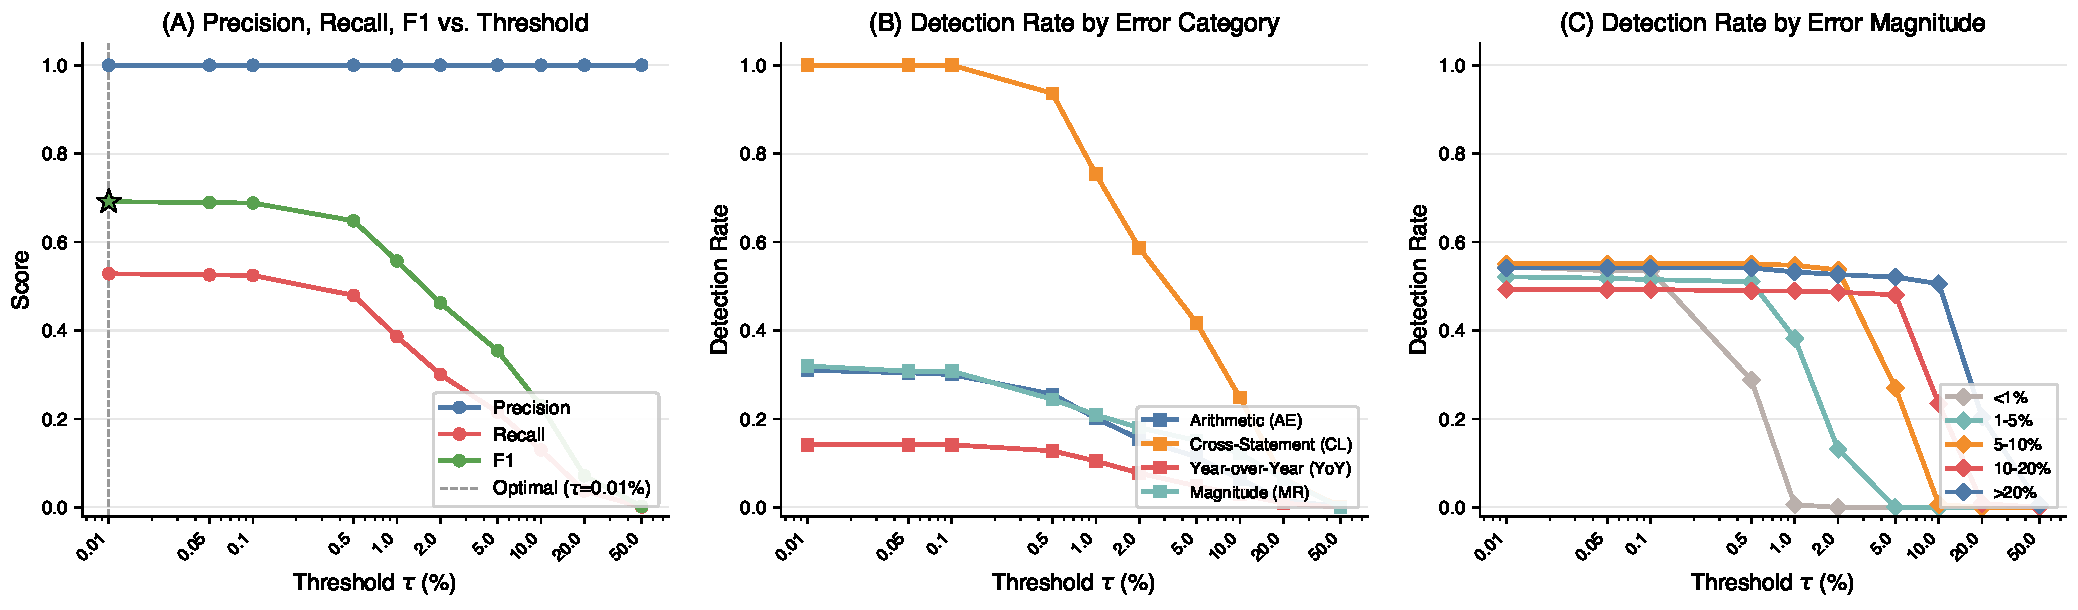
\includegraphics[width=0.95\textwidth]{figures/figure_threshold_sensitivity.pdf}
\caption{Detection performance of the rule-based verifier as a function of threshold $\tau$.
Recall degrades monotonically with increasing threshold, while precision remains at 100\% across all thresholds.
The shaded region marks the ``materiality zone'' (1--5\%) where misstatements may be considered immaterial under SEC guidelines.}
\label{fig:threshold}
\end{figure}

\begin{figure}[t]
\centering
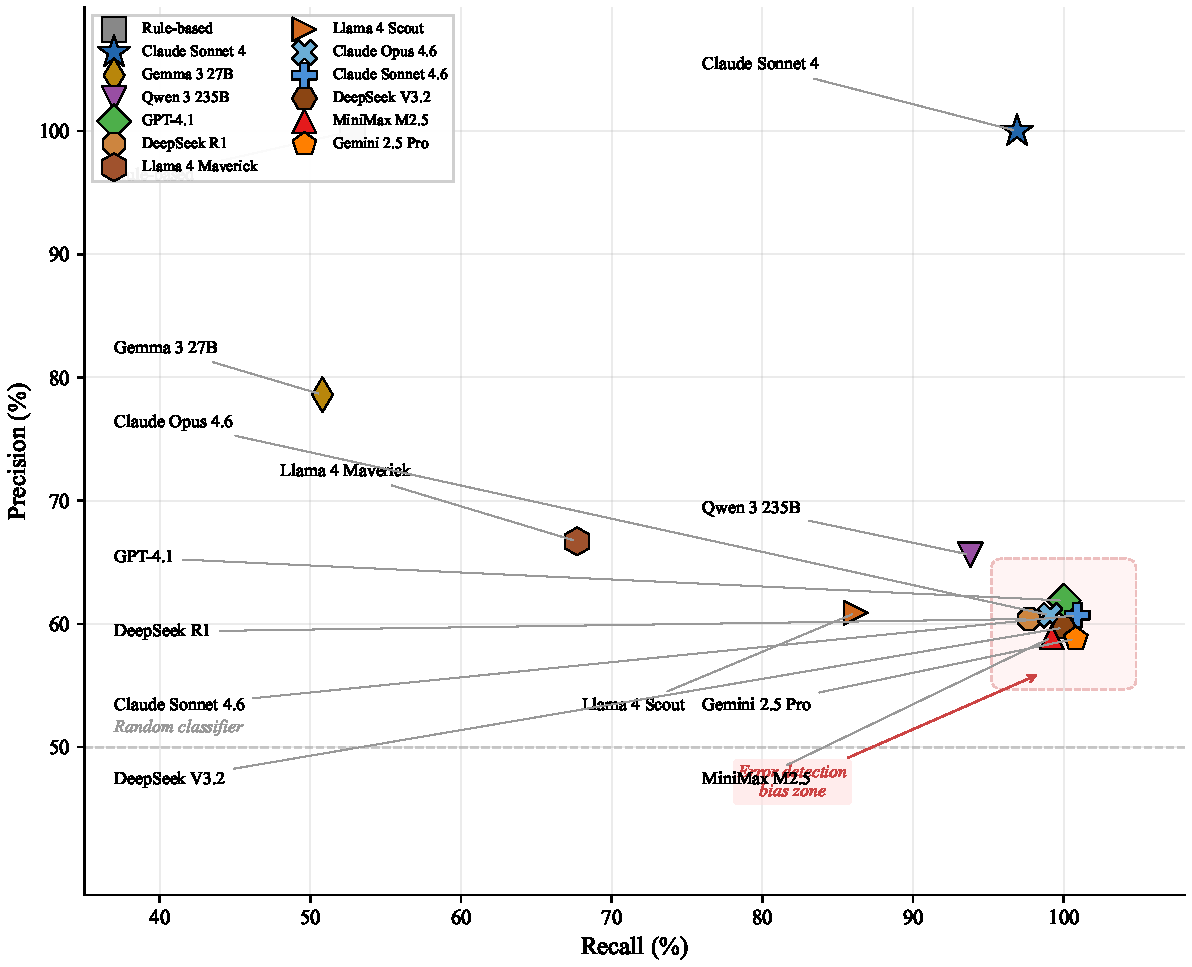
\includegraphics[width=0.85\textwidth]{figures/figure_precision_recall.pdf}
\caption{Precision-recall trade-off across verification systems.
The rule-based verifier occupies the high-precision, low-recall corner; six LLMs cluster in the high-recall, low-precision region (error detection bias zone); Qwen 3 235B and Llama 4 Maverick occupy intermediate positions; and Claude Sonnet 4 uniquely achieves the ideal top-right with 100\% precision and 96.9\% recall.}
\label{fig:precision_recall}
\end{figure}

\subsection{The Verification Gap}
\label{sec:results:noise}

The 47\% of errors that the rule-based verifier misses constitute the \emph{verification gap}---the space of accounting constraints that are not explicitly programmed but that a knowledgeable verifier should check.
This gap arises from two sources:

\paragraph{Partial observability.}
Real financial statements contain dozens of line items per section, with many not captured by standard XBRL concept mappings.
For instance, ``Cash from Investing Activities'' includes capital expenditures, acquisitions, divestitures, and investment sales---but our XBRL extraction captures only capital expenditures.
A rule that checks ``CapEx $=$ Cash from Investing'' would produce discrepancies exceeding 1,000\% on clean data.
We found that when we extend the verifier to check 30 relationships (including these partial-observability rules), recall increases to 100\% but FPR also increases to 100\%---a precision-recall trade-off that cannot be resolved without contextual understanding.

\paragraph{Implicit constraints.}
Some consistency checks require domain knowledge not expressed in the statement structure itself.
For example, verifying that retained earnings changed by exactly (net income $-$ dividends $-$ share repurchases) requires knowing the accounting relationship between these items---knowledge that is implicit rather than explicit in the financial statements.

This analysis has important implications.
The verification gap quantifies the value that a context-aware system (such as an LLM with accounting knowledge) could add over a purely rule-based approach: the ability to check the approximately 47\% of constraints that require either reasoning about incomplete data or implicit domain knowledge.
\benchmark{} is designed to test exactly this capability.

\subsection{Dataset Analysis}
\label{sec:results:dataset}

The benchmark provides systematic coverage across all four error categories (\Cref{tab:dataset_stats}), with up to 46 error-injected instances per company spanning 7 non-magnitude error subtypes at 6 magnitude levels (42) plus 4 magnitude-category instances.
\begin{figure}[t]
\centering
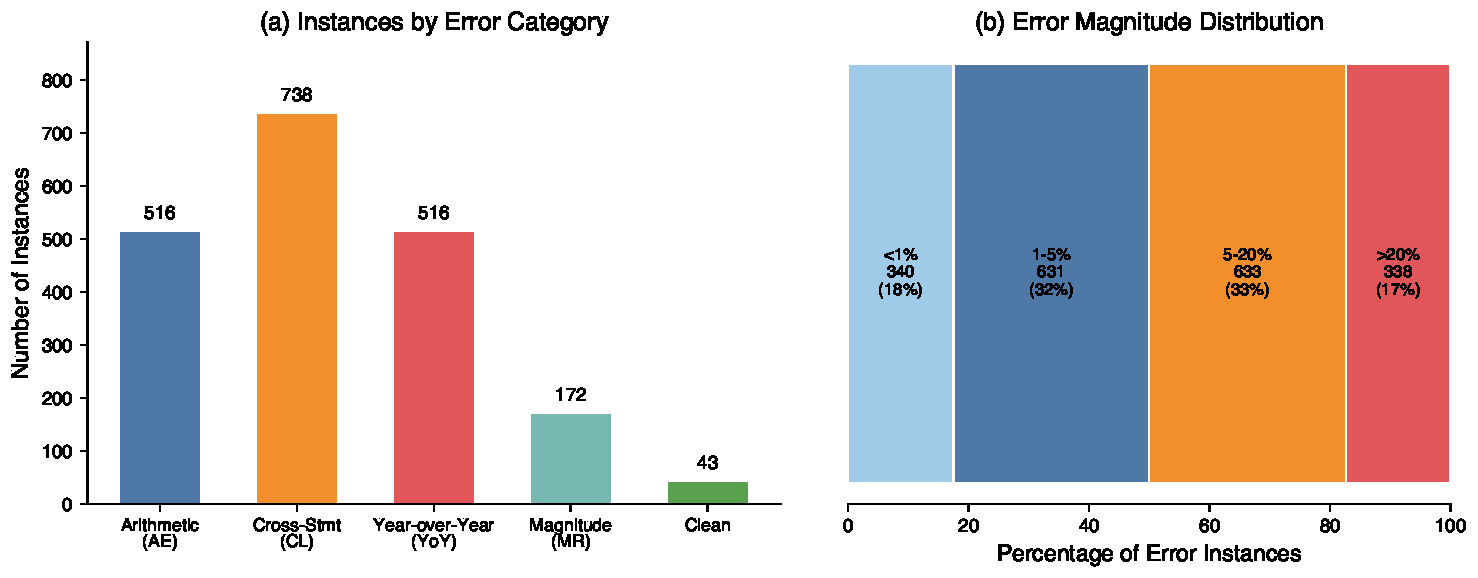
\includegraphics[width=0.9\textwidth]{figures/figure_dataset_composition.pdf}
\caption{Dataset composition of \benchmark{}.
Left: number of instances by error category (AE = arithmetic, CL = cross-statement, YoY = year-over-year, MR = magnitude/rounding).
Right: distribution of error magnitudes across the benchmark.}
\label{fig:dataset_composition}
\end{figure}

\Cref{fig:dataset_composition} shows the distribution of instances across error categories and magnitudes.
The 43 companies span 8 sectors: technology (15), healthcare/pharma (6), consumer goods (5), financial services (4), industrials (4), energy (3), telecommunications (3), and other (3) (\Cref{fig:diversity}).
This sectoral diversity ensures that the benchmark captures variation in financial reporting practices across industries.

\begin{figure}[t]
\centering
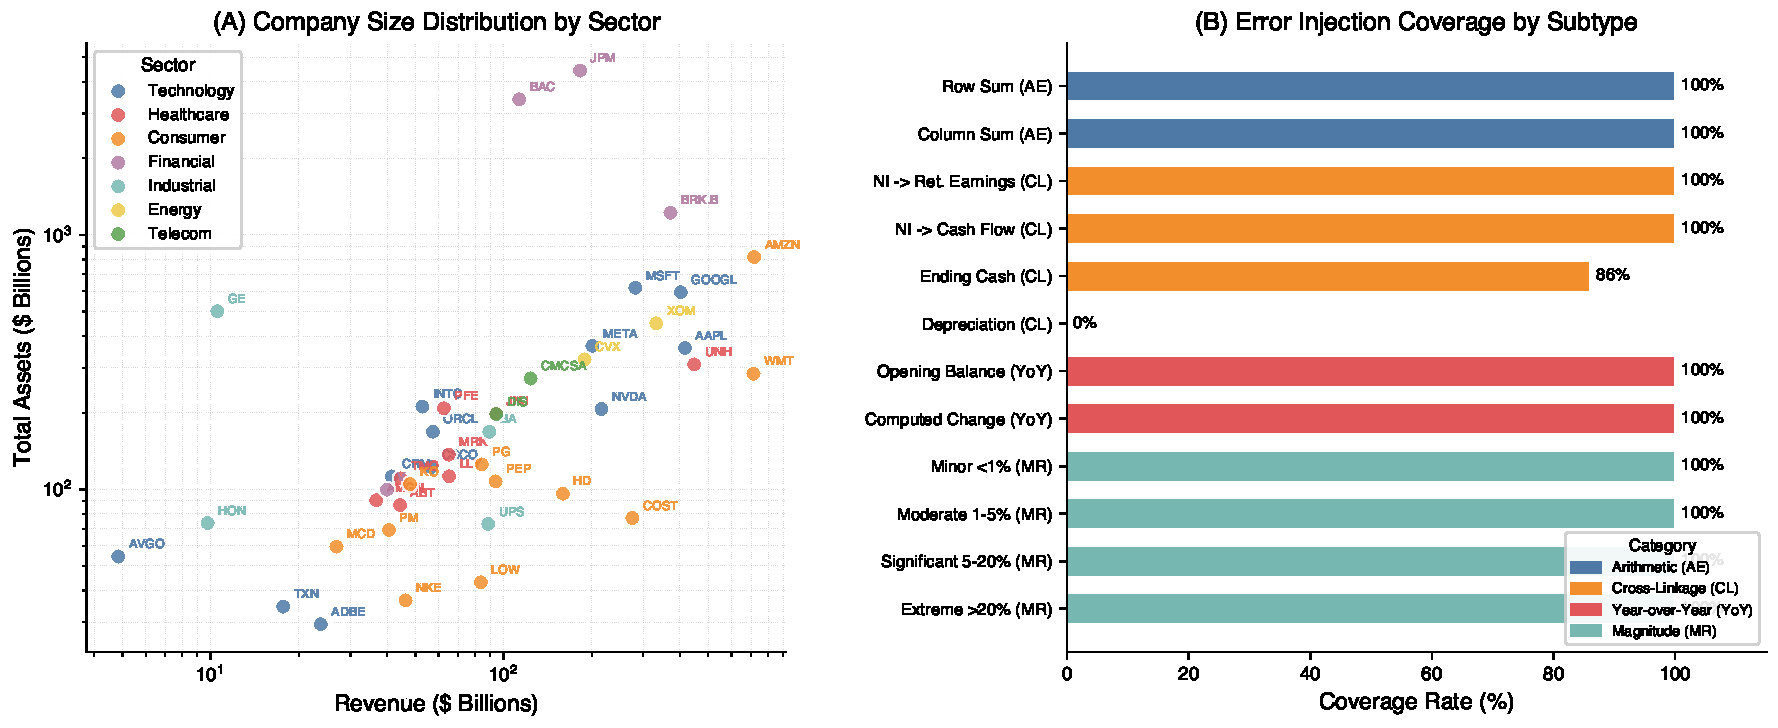
\includegraphics[width=0.85\textwidth]{figures/figure_dataset_diversity.pdf}
\caption{Left: Revenue vs.\ total assets for the 43 companies in \benchmark{} (log-log scale, colored by sector), showing the wide range of company sizes and financial profiles covered.
Right: Error injection coverage rate by error subtype; 10 of 12 subtypes achieve 100\% coverage.}
\label{fig:diversity}
\end{figure}

The companies span a wide range of financial profiles: revenue from \$4.8B to \$716.9B (median \$84.3B) and total assets from \$29.5B to \$4.4T (median \$136.9B), with an average of 12.2 checkable accounting relationships per company (\Cref{fig:diversity}).
All 43 companies have complete data for all three financial statements and prior-year comparatives, ensuring full coverage of year-over-year error types.
10 of 12 error subtypes achieve 100\% injection coverage; CL-Ending Cash covers 86\% (37/43), while CL-D\&A could not be injected for any company due to depreciation being reported only on the cash flow statement in XBRL filings.

\begin{figure}[t]
\centering
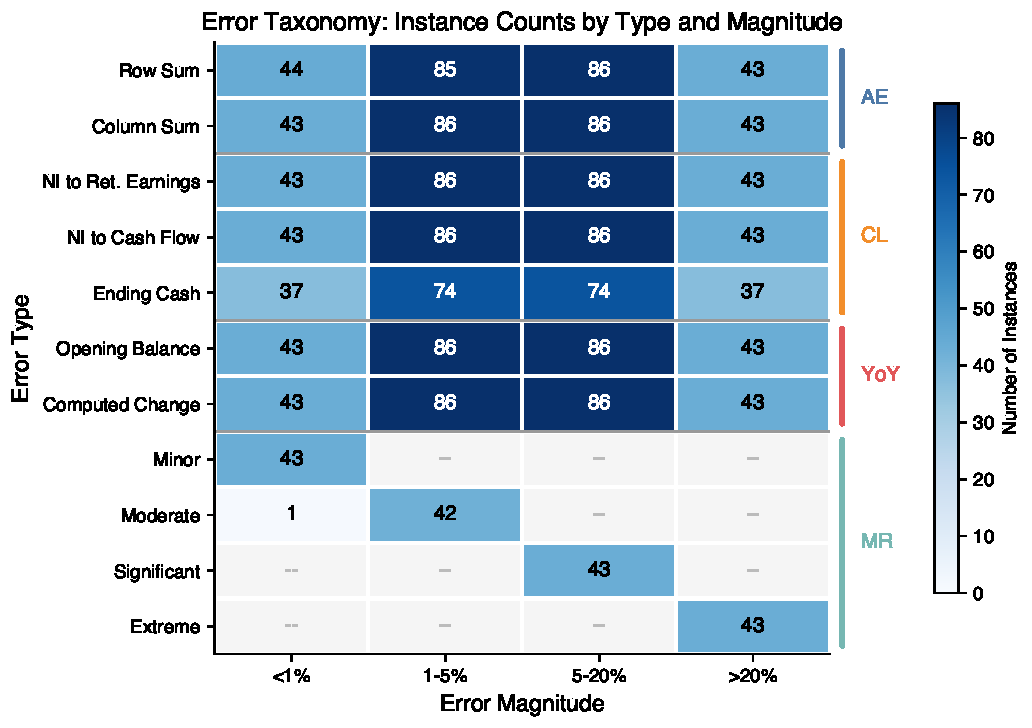
\includegraphics[width=0.95\textwidth]{figures/figure_error_taxonomy.pdf}
\caption{Heatmap of benchmark instances by error type (rows) and magnitude level (columns). Each cell shows the number of instances, enabling systematic analysis of detection sensitivity across the full error type $\times$ magnitude grid.}
\label{fig:taxonomy_heatmap}
\end{figure}

The error type $\times$ magnitude grid (\Cref{fig:taxonomy_heatmap}) confirms uniform coverage across cells, enabling fine-grained sensitivity analysis.

\subsection{Benchmark Validation}
\label{sec:results:validation}

We validate the benchmark through several checks:

\paragraph{Error injection fidelity.}
For each injected error, we verify that (a) exactly one line item was modified, (b) the modification matches the specified magnitude within rounding tolerance, and (c) the ground truth correctly records the original and modified values.
All 1,942 error instances pass these checks.

\paragraph{Clean instance consistency.}
Clean instances are verified against the fundamental accounting identity ($\text{Assets} = \text{Liabilities} + \text{Equity}$) and inter-statement linkages that we explicitly construct (IS net income $=$ CFS net income; CFS ending cash $=$ BS cash).
All 43 clean instances satisfy these core constraints.

\paragraph{Error discriminability.}
We verify that error-injected instances are distinguishable from clean instances at their injected error location.
The minimum absolute perturbation across all instances is \$0.5M (at 0.5\% magnitude for small line items), confirming that all errors exceed rounding precision.

\subsection{Framework for LLM Evaluation}
\label{sec:results:framework}

\benchmark{} includes a complete evaluation framework for LLM-based verification.
We provide prompt templates for two strategies (\Cref{app:prompts}):

\paragraph{Zero-shot.}
The model receives financial statements and a general verification instruction.
This tests whether models can identify inconsistencies without explicit guidance on what to check.

\paragraph{Chain-of-thought (CoT).}
The model is instructed to systematically check specific accounting relationships step by step, mirroring audit procedures.
This tests whether structured reasoning improves detection, particularly for cross-statement errors that require maintaining relationships across document sections.
The framework also includes a few-shot template (not evaluated in this study) for future prompting strategy ablations.

\subsection{LLM Evaluation}
\label{sec:results:llm}

\Cref{tab:llm_results} presents results from evaluating twelve frontier LLMs---Claude Sonnet~4~\citep{claude2025} ($n=108$), Claude Opus~4.6 ($n=108$), Claude Sonnet~4.6 ($n=108$), GPT-4.1~\citep{openai2025gpt41} ($n=108$), DeepSeek V3.2~\citep{deepseek2025v3} ($n=108$), DeepSeek R1 ($n=108$), Qwen 3 235B~\citep{qwen2025qwen3} ($n=108$), Llama 4 Maverick~\citep{meta2025llama4} ($n=108$), Llama 4 Scout ($n=108$), Gemma 3 27B ($n=108$), Gemini 2.5 Pro~\citep{google2025gemini} ($n=68$ valid), and MiniMax~M2.5~\citep{minimax2025} ($n=90$)---on stratified samples from the benchmark.

\begin{table}[t]
\centering
\footnotesize
\caption{Comparison of the rule-based verifier and twelve frontier LLMs on \benchmark{}.
95\% Wilson confidence intervals shown in brackets.
$n$: number of evaluation instances with valid responses.
Eleven of twelve models evaluated under CoT prompting; MiniMax under zero-shot.
$^\dagger$Gemini: 40/108 API calls returned server errors; metrics on 68 valid responses.
}
\label{tab:llm_results}
\begin{tabular}{llccccccc}
\toprule
\textbf{System} & \textbf{Strategy} & $\bm{n}$ & \textbf{Acc.} & \textbf{Prec.} & \textbf{Rec.} & \textbf{F1} & \textbf{FPR} & \textbf{Loc.} \\
\midrule
Rule-based & $\tau=0.01\%$ & 1985 & 53.8 & 100.0 & 52.8 & 69.1 & 0.0 & 62.6 \\
\midrule
Claude Sonnet 4 & CoT & 108 & \textbf{98.1} & \textbf{100.0} & 96.9 & \textbf{98.4} & \textbf{0.0} & \textbf{100.0} \\
 & & & \scriptsize{[93.5, 99.5]} & \scriptsize{[94.3, 100]} & \scriptsize{[89.5, 99.2]} &  & \scriptsize{[0, 8.2]} & \\
Gemma 3 27B & CoT & 108 & 62.0 & 78.6 & 50.8 & 61.7 & 20.9 & 93.9 \\
 & & & \scriptsize{[52.6, 70.7]} & \scriptsize{[66.2, 87.5]} & \scriptsize{[38.9, 62.6]} &  & \scriptsize{[11.4, 35.2]} & \\
Qwen 3 235B & CoT & 108 & 66.7 & 65.6 & 93.8 & 77.2 & 74.4 & 85.2 \\
 & & & \scriptsize{[57.3, 75.0]} & \scriptsize{[55.7, 74.4]} & \scriptsize{[85.0, 97.5]} & & \scriptsize{[60.2, 85.0]} & \\
GPT-4.1 & CoT & 108 & 62.0 & 61.3 & \textbf{100.0} & 76.0 & 95.3 & 70.8 \\
 & & & \scriptsize{[52.6, 70.7]} & \scriptsize{[52.2, 69.8]} & \scriptsize{[94.4, 100]} & & \scriptsize{[84.5, 98.7]} & \\
DeepSeek R1 & CoT & 108 & 61.1 & 61.0 & 98.5 & 75.3 & 95.3 & 60.7 \\
 & & & \scriptsize{[51.7, 69.8]} & \scriptsize{[51.6, 69.6]} & \scriptsize{[91.8, 99.7]} & & \scriptsize{[84.5, 98.7]} & \\
Cl.\ Opus 4.6 & CoT & 108 & 60.2 & 60.2 & \textbf{100.0} & 75.1 & 100.0 & 78.5 \\
 & & & \scriptsize{[50.8, 68.8]} & \scriptsize{[50.8, 68.8]} & \scriptsize{[94.4, 100]} & & \scriptsize{[91.8, 100]} & \\
Cl.\ Sonnet 4.6 & CoT & 108 & 60.2 & 60.2 & \textbf{100.0} & 75.1 & 100.0 & 73.8 \\
 & & & \scriptsize{[50.8, 68.8]} & \scriptsize{[50.8, 68.8]} & \scriptsize{[94.4, 100]} & & \scriptsize{[91.8, 100]} & \\
DeepSeek V3.2 & CoT & 108 & 60.2 & 60.2 & \textbf{100.0} & 75.1 & 100.0 & 86.2 \\
 & & & \scriptsize{[50.8, 68.8]} & \scriptsize{[50.8, 68.8]} & \scriptsize{[94.4, 100]} & & \scriptsize{[91.8, 100]} & \\
Llama 4 Maverick & CoT & 108 & 60.2 & 66.7 & 67.7 & 67.2 & 51.2 & 84.1 \\
 & & & \scriptsize{[50.8, 68.8]} & \scriptsize{[54.7, 76.8]} & \scriptsize{[55.6, 77.8]} & & \scriptsize{[36.8, 65.4]} & \\
Llama 4 Scout & CoT & 108 & 58.3 & 60.9 & 86.2 & 71.3 & 83.7 & 82.1 \\
 & & & \scriptsize{[48.8, 67.1]} & \scriptsize{[51.3, 69.7]} & \scriptsize{[75.7, 92.5]} & & \scriptsize{[70.0, 92.0]} & \\
MiniMax M2.5 & Zero-shot & 90 & 58.9 & 58.9 & \textbf{100.0} & 74.1 & 100.0 & --- \\
 & & & \scriptsize{[48.8, 68.3]} & \scriptsize{[48.8, 68.3]} & \scriptsize{[93.4, 100]} & & \scriptsize{[89.3, 100]} & \\
Gemini 2.5 Pro$^\dagger$ & CoT & 68 & 58.8 & 58.8 & \textbf{100.0} & 74.1 & 100.0 & 85.0 \\
 & & & \scriptsize{[47.2, 69.6]} & \scriptsize{[47.2, 69.6]} & \scriptsize{[91.2, 100]} & & \scriptsize{[85.4, 100]} & \\
\bottomrule
\end{tabular}
\end{table}

\paragraph{Finding 1: the central challenge is calibration, not detection.}
The most striking result is the wide \emph{calibration spectrum} across models that otherwise achieve high recall.
Claude Sonnet 4 achieves \textbf{98.1\% accuracy} with \textbf{perfect precision} (0\% FPR) and \textbf{96.9\% recall}, correctly identifying 63 of 65 injected errors while producing zero false positives across all 43 clean instances.
At the other extreme, five models achieve \textbf{100\% FPR} across all evaluated instances: Claude Opus 4.6, Claude Sonnet 4.6, DeepSeek V3.2, MiniMax M2.5, and Gemini 2.5 Pro.
GPT-4.1 achieves \textbf{100\% recall} with \textbf{95.3\% FPR} (flagging 41 of 43 clean instances).
Between these extremes, four models show intermediate calibration.
Gemma 3 27B achieves a \textbf{conservative} profile: 50.8\% recall with only 20.9\% FPR---the second-lowest FPR after Claude, but at a significant recall cost, with the highest precision (78.6\%) among non-calibrated models and 93.9\% localization accuracy.
Llama 4 Maverick occupies a \textbf{moderate} position: 67.7\% recall with 51.2\% FPR.
Qwen 3 235B achieves \textbf{partial calibration}: 93.8\% recall with 74.4\% FPR (correctly identifying 11 of 43 clean instances).
Llama 4 Scout shows \textbf{near-biased} behavior: 86.2\% recall with 83.7\% FPR, notably weaker than its sibling Maverick, demonstrating intra-family calibration variation within Meta's model line.
This spectrum---from 0\% to 100\% FPR---spans seven independent providers and both closed-source and open-weight architectures, establishing that calibration quality varies continuously.
These systems occupy fundamentally different positions in the precision-recall space (\Cref{fig:precision_recall}), with Claude Sonnet 4 uniquely achieving the calibrated judgment that practical deployment requires.

\begin{figure}[t]
\centering
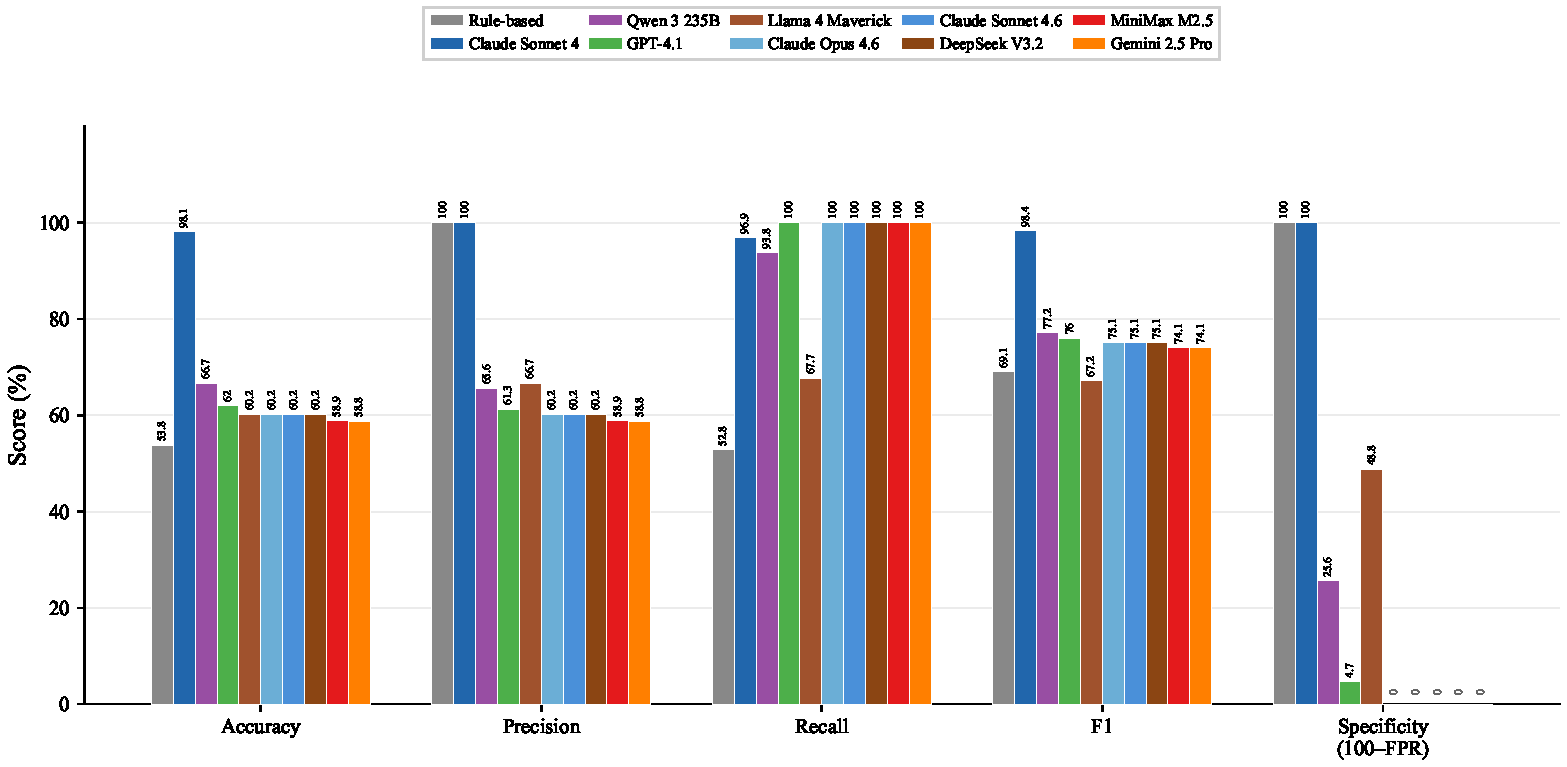
\includegraphics[width=0.95\textwidth]{figures/figure_model_comparison_updated.pdf}
\caption{Comparison of all verification systems across five metrics.
Ten of twelve LLMs achieve $\geq$86\% recall; Gemma 3 27B and Llama 4 Maverick trade recall for higher precision.
Only Claude Sonnet 4 combines high recall with low FPR.
Only Claude Sonnet 4 achieves low FPR (0\%) and high accuracy (98.1\%).}
\label{fig:model_comparison}
\end{figure}

\paragraph{Finding 2: Claude Sonnet 4 achieves near-perfect error detection and localization.}
\Cref{tab:category_results} shows Claude's detection rates by error category.
Claude achieves \textbf{100\% detection} on both arithmetic errors (AE) and cross-statement linkage violations (CL)---the two categories that require systematic checking of numerical relationships.
Detection is slightly lower for year-over-year consistency errors (93.8\%) and magnitude perturbations (88.9\%).
Notably, Claude achieves \textbf{100\% localization accuracy}: for every detected error, it correctly identifies the specific line item that was modified.

\begin{table}[t]
\centering
\footnotesize
\caption{Detection rate (\%) by error category.
Ten of twelve LLMs achieve $\geq$86\% recall, but seven achieve this at the cost of high FPR (95--100\%), flagging nearly all clean instances as erroneous.
Only Claude Sonnet 4 achieves selective detection with 0\% FPR.
$^\dagger$Gemini metrics on 68 valid responses (37\% API error rate).
}
\label{tab:category_results}
\begin{tabular}{lrrrrrrrrrrrr}
\toprule
\textbf{Cat.} & $\bm{n}$ & \textbf{Cl.S4} & \textbf{Gem3} & \textbf{Qwen} & \textbf{GPT} & \textbf{R1} & \textbf{Mav} & \textbf{Sct} & \textbf{Biased$^*$} & \textbf{Rule} \\
\midrule
AE       & 16 & 100.0 & 25.0 & 93.8 & 100.0 & 100.0 & 43.8 & 87.5 & 100.0 & 31.0 \\
CL  & 24 & 100.0 & 75.0 & 95.8 & 100.0 & 95.8 & 87.5 & 83.3 & 100.0 & 100.0 \\
YoY  & 16 & 93.8 & 37.5 & 87.5 & 100.0 & 100.0 & 62.5 & 87.5 & 100.0 & 14.2 \\
MR        &  9 & 88.9 & 55.6 & 100.0 & 100.0 & 100.0 & 66.7 & 88.9 & 100.0 & 32.0 \\
\midrule
\textbf{Overall}      & 65 & \textbf{96.9} & 50.8 & 93.8 & 100.0 & 98.5 & 67.7 & 86.2 & 100.0 & 52.8 \\
\midrule
\textbf{Clean}  & 43 & \textbf{100.0} & 79.1 & 25.6 & 4.7 & 4.7 & 48.8 & 16.3 & 0.0 & 100.0 \\
\bottomrule
\multicolumn{10}{l}{\scriptsize $^*$Biased = Cl.~Opus~4.6, Cl.~Sonnet~4.6, DeepSeek V3.2, Gemini 2.5 Pro, MiniMax M2.5 (all 100\% on all categories).}
\end{tabular}
\end{table}

\paragraph{Finding 3: detection is robust across error magnitudes.}
\Cref{tab:magnitude_results} presents detection rates by error magnitude.
Remarkably, Claude detects errors at \textbf{100\% even below the 1\% magnitude level}---well below the SEC's 5\% materiality presumption threshold.
Detection rates are slightly lower at larger magnitudes (93.8\% for both 5--20\% and $>$20\%), where the two missed errors involve a year-over-year opening balance discrepancy and an extreme magnitude perturbation.
This pattern---high detection at small magnitudes, slightly lower at large (\Cref{fig:magnitude_curves})---is counterintuitive and suggests that Claude's verification relies on structural relationship checking rather than magnitude scanning.

\begin{table}[t]
\centering
\small
\caption{Detection rate by error magnitude with 95\% Wilson CIs.
Claude Sonnet 4 achieves perfect detection at small magnitudes ($<5\%$), with only two misses at larger magnitudes.
Qwen 3 235B is the only other model with non-trivial magnitude sensitivity.
Six biased models (not shown) achieve 100\% across all magnitudes trivially (at 95--100\% FPR).
The rule-based verifier's recall is approximately constant because detection depends on \emph{which} relationship is checked, not the perturbation size.}
\label{tab:magnitude_results}
\begin{tabular}{lrrrr}
\toprule
\textbf{Magnitude} & $\bm{n}$ & \textbf{Cl.\ Sonnet 4 (\%)} & \textbf{Qwen 3 (\%)} & \textbf{Rule (\%)} \\
\midrule
$<1\%$   & 17 & 100.0 {\scriptsize [81.6, 100]} & 88.2 & 52.8 \\
$1$--$5\%$  & 16 & 100.0 {\scriptsize [80.6, 100]} & 93.8 & 52.8 \\
$5$--$20\%$ & 16 & 93.8 {\scriptsize [71.7, 98.9]}  & 100.0 & 52.8 \\
$>20\%$  & 16 & 93.8 {\scriptsize [71.7, 98.9]}  & 93.8 & 52.8 \\
\bottomrule
\end{tabular}
\end{table}

\begin{figure}[t]
\centering
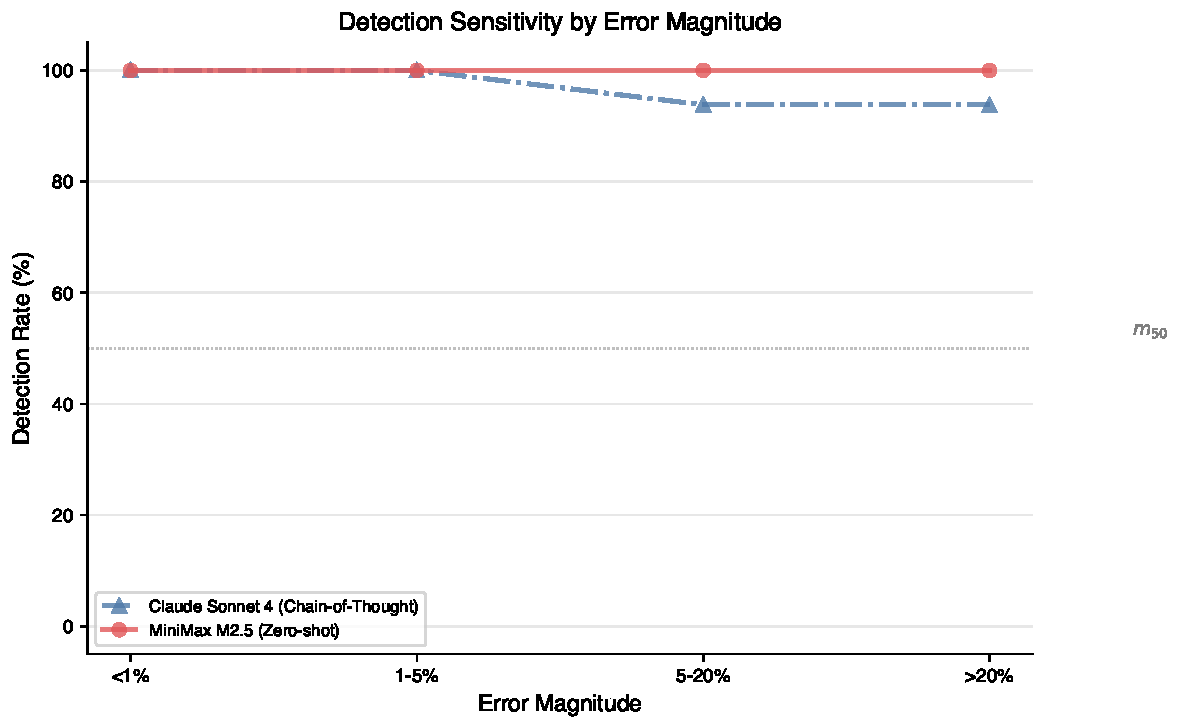
\includegraphics[width=0.9\textwidth]{figures/figure_magnitude_curves.pdf}
\caption{Detection sensitivity by error magnitude.
Claude Sonnet 4 achieves 100\% detection at magnitudes below 5\% (the SEC materiality presumption threshold), with only slight degradation at larger magnitudes.
The dotted line marks the $m_{50}$ threshold (50\% detection rate).}
\label{fig:magnitude_curves}
\end{figure}

\paragraph{Finding 4: error detection bias is the default LLM behavior.}
Seven of twelve LLMs exhibit strong \emph{error detection bias}: when instructed to examine for errors, these models find discrepancies in nearly every financial statement, including those without injected errors.
Five models achieve 100\% FPR---Claude Opus 4.6, Claude Sonnet 4.6, DeepSeek V3.2, Gemini 2.5 Pro, and MiniMax M2.5---flagging every clean instance as erroneous.
GPT-4.1 and DeepSeek R1 each flag 41 of 43 clean instances (FPR = 95.3\%).
Notably, DeepSeek R1 is a reasoning-specialized model with explicit chain-of-thought capabilities, yet achieves the same FPR as GPT-4.1 and the lowest localization accuracy of any model (60.7\%), suggesting that reasoning depth does not improve verification calibration.
This is particularly notable for three reasons.
First, six of the eleven CoT-evaluated models with the standard prompt share the \emph{identical} prompt, ruling out prompting strategy as the explanation.
Second, MiniMax exhibits the same bias under all three tested strategies (zero-shot, few-shot, CoT), confirming prompt independence.
Third---and most strikingly---Claude Opus 4.6 and Sonnet 4.6, from the \emph{same provider} as the calibrated Claude Sonnet 4, both exhibit 100\% FPR, demonstrating that error detection bias can emerge \emph{within a model family} across generations.
Manual inspection reveals that all biased models identify \emph{genuine but benign} discrepancies arising from partial observability in the data---the same issues discussed in \Cref{sec:results:noise}.
For GPT-4.1, false positives typically involve miscomputing operating income from an abbreviated statement that omits certain line items (e.g., stock-based compensation).
Among non-calibrated models, localization accuracy on true positives varies widely: Gemma 3 93.9\%, DeepSeek V3.2 86.2\%, Qwen 85.2\%, Gemini 85.0\%, Llama 4 Maverick 84.1\%, Scout 82.1\%, Claude Opus 4.6 78.5\%, Claude Sonnet 4.6 73.8\%, GPT-4.1 70.8\%, and DeepSeek R1 60.7\%---suggesting that even when models correctly detect an injected error, they frequently attribute it to the wrong field.
Claude Sonnet 4, by contrast, demonstrates the calibrated judgment needed to distinguish injected errors from expected rounding discrepancies, achieving a 0\% false positive rate [95\% CI: 0--8.2\%] with 100\% localization accuracy.
The observation that non-calibrated behavior (FPR $>$ 0\%) appears across all seven evaluated providers (Anthropic, OpenAI, DeepSeek, Google, Alibaba/Qwen, Meta, MiniMax), across prompting strategies (CoT, zero-shot), and \emph{within} four model families (Anthropic, DeepSeek, Meta, Google), establishes this as a fundamental challenge for LLMs in verification tasks.
\Cref{fig:category_heatmap} visualizes detection rates across error categories and systems, highlighting the contrast between universal error recall and divergent clean-instance specificity.

\begin{figure}[t]
\centering
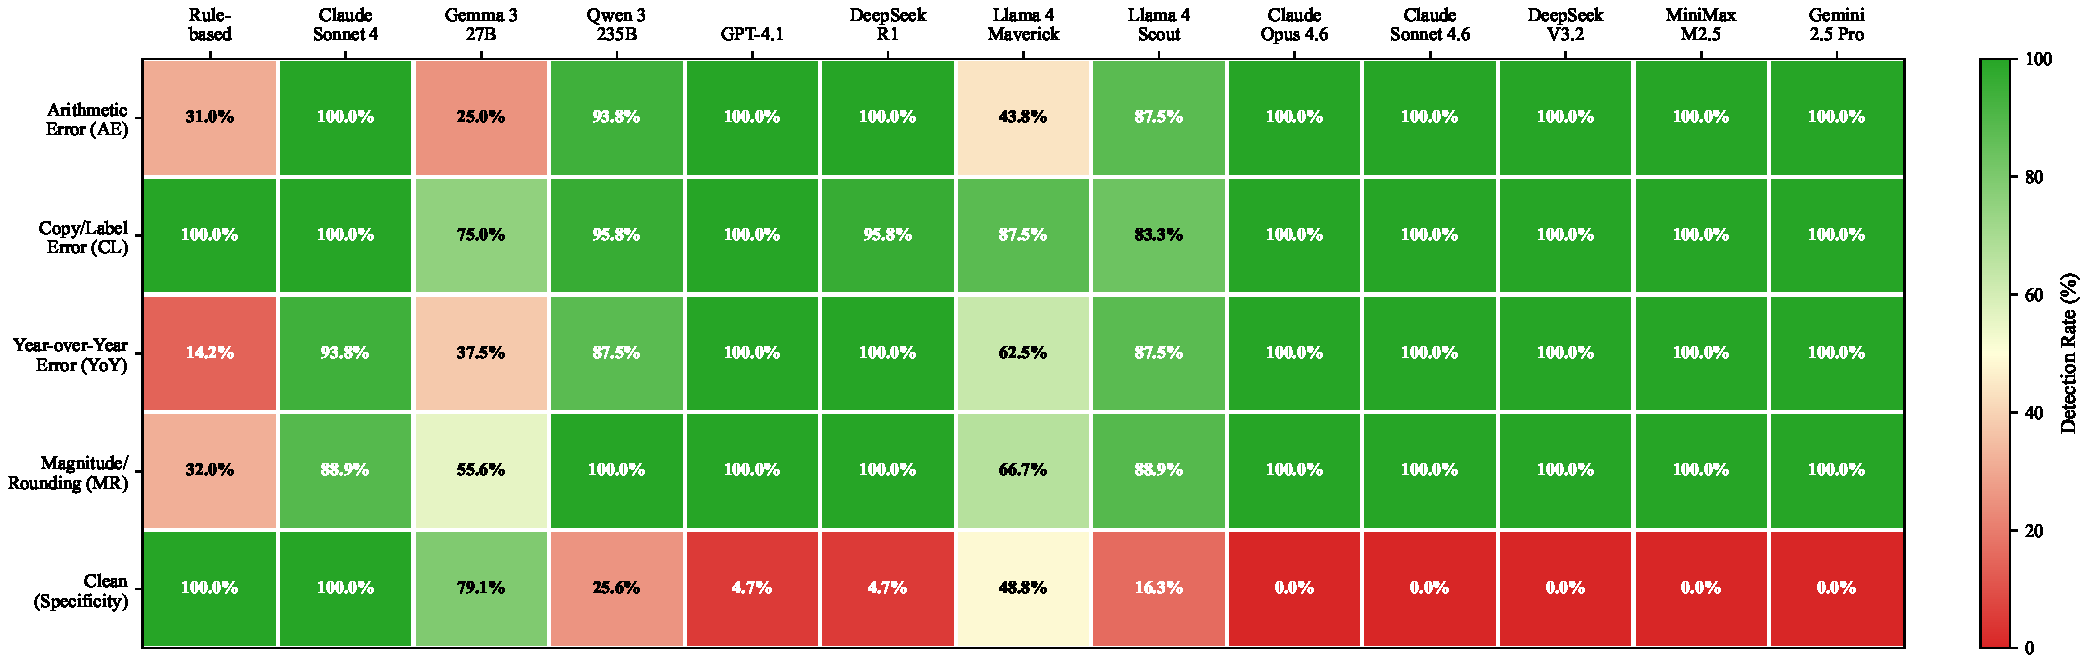
\includegraphics[width=0.85\textwidth]{figures/figure_category_heatmap_updated.pdf}
\caption{Detection rate heatmap by error category and system.
Most LLMs achieve high recall across error categories, but Llama 4 Maverick shows category-specific weakness (AE: 43.8\%).
Models differ dramatically on clean instances (bottom row): only Claude Sonnet 4 and the rule-based verifier achieve full specificity.}
\label{fig:category_heatmap}
\end{figure}

\paragraph{Finding 5: false negative analysis reveals benchmark limitations.}
The calibrated model's two false negatives are both cases where the error was injected into a field \emph{not displayed} in the formatted financial statements.
The MR\_EXTREME miss involved a 25\% perturbation to goodwill---a field not broken out as a separate line item in our balance sheet format.
The YoY miss modified prior-year shares outstanding, which is similarly not displayed.
In both cases, the model correctly verified all \emph{visible} relationships and reported no inconsistencies.
While this \emph{suggests} the errors may have been undetectable from the presented data, we note that this is a post-hoc observation and cannot be treated as definitive evidence of perfect verification capability.
This finding highlights an important benchmark design consideration: error injection into non-displayed fields creates instances that may be inherently unsolvable, and future benchmark versions should ensure all injected errors are detectable from the visible data.

\paragraph{Implications and caveats.}
These results reveal that financial verification performance varies widely across frontier LLMs, even when evaluated under identical conditions.
The paired comparison between Claude Sonnet 4 and GPT-4.1 is particularly informative: both are evaluated on the same 108 instances under the same CoT prompt, isolating model capability from prompting effects.
The 36-percentage-point accuracy gap (98.1\% vs.\ 62.0\%) and the FPR difference (0\% [95\% CI: 0--8.2\%] vs.\ 95.3\%) cannot be attributed to prompting differences and are highly significant (McNemar's $p < 10^{-9}$; \Cref{sec:analysis:significance}).
We note that Claude Sonnet 4's 0\% FPR, while striking, is based on only 43 clean instances; the 95\% Wilson CI upper bound of 8.2\% means a small but non-zero FPR cannot be ruled out.
The practical implication is that deploying \emph{any} LLM for financial verification without task-specific evaluation on a benchmark like \benchmark{} risks either excellent or catastrophically poor calibration---and that even success on one model version does not guarantee success on the next.

% ==============================================================================
\section{Analysis}
\label{sec:analysis}
% ==============================================================================

\subsection{What Makes Financial Verification Hard?}
\label{sec:analysis:hard}

Our benchmark construction and baseline analysis reveal several factors that make financial statement verification fundamentally challenging:

\paragraph{Incomplete information.}
Real financial statements contain dozens of line items per section, but standardized XBRL taxonomies capture only a subset.
Our analysis of 43 S\&P 500 companies shows that simplified summation relationships (e.g., ``capital expenditures $=$ cash from investing'') can diverge by over 1,000\% from reality because of unmodeled components (acquisitions, divestitures, investment sales).
Any verifier---rule-based or LLM---must reason about what it \emph{cannot} see.

\paragraph{Numerical precision and rounding.}
Financial statements report figures rounded to the nearest million or thousand.
At the 0.5\% magnitude level, the absolute difference between the correct and erroneous values can be as small as \$0.5M for a \$100M line item---comparable to the rounding unit itself.
This creates an inherent ambiguity zone where verification is genuinely underdetermined.

\paragraph{Cross-document reasoning.}
Cross-statement errors (CL category) require maintaining and comparing numerical values across three separate document sections (income statement, balance sheet, cash flow statement)---a task that existing benchmarks on numerical reasoning over long documents~\citep{zhao2024docmatheval} have shown to degrade LLM performance significantly.

\paragraph{Implicit domain knowledge.}
Some verification checks require knowledge of accounting relationships that are not stated in the input.
For example, detecting a CL-NI/RE error requires knowing that net income should flow to retained earnings minus dividends---a fundamental accounting relationship but one that is implicit rather than explicitly stated in the financial statements.
The chain-of-thought prompt partially addresses this by making key relationships explicit, but the set of possible relationships is large and domain-specific.

\subsection{The Precision-Recall Spectrum in Financial Verification}
\label{sec:analysis:rulevllm}

Our results reveal a spectrum of verification behaviors across six LLM archetypes (plus the rule-based baseline):

\begin{itemize}[topsep=2pt,itemsep=1pt]
    \item \textbf{Rule-based (deterministic)}: By restricting checks to relationships that hold exactly in clean data, the verifier achieves 0\% FPR but only 52.8\% recall---missing errors that violate unchecked relationships.
    \item \textbf{Biased (7 models)}: Claude Opus 4.6, Claude Sonnet 4.6, DeepSeek V3.2, DeepSeek R1, Gemini 2.5 Pro, MiniMax M2.5, and GPT-4.1 all achieve 95--100\% FPR, identifying nearly every financial statement as inconsistent.
    GPT-4.1 and DeepSeek R1 each correctly identify 2 of 43 clean instances; the other five flag every clean instance as erroneous.
    \item \textbf{Llama 4 Scout (near-biased)}: Achieves 86.2\% recall with 83.7\% FPR, positioned between the biased cluster and the partially calibrated models.
    Notably weaker than its sibling Maverick (51.2\% FPR), demonstrating calibration variability within Meta's model family.
    \item \textbf{Qwen 3 235B (partially calibrated)}: Achieves 93.8\% recall with 74.4\% FPR, correctly identifying 11 of 43 clean instances.
    Maintains high recall while beginning to exercise selective judgment.
    \item \textbf{Llama 4 Maverick (moderate)}: Achieves 67.7\% recall with 51.2\% FPR, genuinely trading recall for specificity.
    Excels on cross-statement linkage errors (87.5\%) but struggles with arithmetic column sums (43.8\%), revealing category-specific verification capabilities.
    \item \textbf{Gemma 3 27B (conservative)}: Achieves 50.8\% recall with only 20.9\% FPR---the most conservative LLM.
    Excels on cross-statement errors (75.0\%) but detects only 25.0\% of arithmetic errors, suggesting reliance on a narrow set of well-known accounting relationships.
    Achieves the highest localization accuracy (93.9\%) among non-calibrated models.
    \item \textbf{Claude Sonnet 4 (fully calibrated)}: Achieves 100\% precision \emph{and} 96.9\% recall, successfully distinguishing injected errors from expected rounding discrepancies.
\end{itemize}

The contrast across all twelve LLMs is particularly illuminating.
All eleven CoT-evaluated models process the same financial statements, yet only Claude Sonnet 4 correctly classifies all 43 clean instances.
With seven of twelve frontier models from five of the seven evaluated providers exhibiting error detection bias---including two \emph{from the same provider} as the calibrated model---we conclude that this is the \emph{default} LLM behavior for verification tasks.
Flagging everything as suspicious is the ``safe'' response when asked to look for errors, and calibrated behavior is the \emph{exception}.
The key capability that Claude Sonnet 4 uniquely demonstrates is \emph{tolerance for expected imprecision}---the ability to recognize that financial statements reported in millions of dollars will have minor rounding discrepancies that do not constitute genuine errors.

\subsection{Statistical Significance and Paired Analysis}
\label{sec:analysis:significance}

Since Claude Sonnet 4 and GPT-4.1 were evaluated on the \emph{same} 108 instances under the \emph{same} CoT prompt, we apply McNemar's test for paired nominal data~\citep{mcnemar1947} to assess whether the performance difference is statistically significant.

\Cref{tab:mcnemar} presents the $2 \times 2$ contingency table of correct/incorrect predictions.
Of 108 instances, 65 are concordant (both models correct on all 65 error instances where GPT-4.1 also correctly detects errors), 41 are discordant in Claude's favor (Claude correct, GPT-4.1 wrong---all clean instances that GPT-4.1 false-alarms on), and only 2 are discordant in GPT-4.1's favor (GPT-4.1 detects an error that Claude misses).

\begin{table}[t]
\centering
\small
\caption{McNemar's test: Claude Sonnet 4 vs.\ GPT-4.1 on the same 108 instances.
The 41:2 discordant split is highly significant ($p < 10^{-9}$), driven entirely by GPT-4.1's false positives on clean instances.}
\label{tab:mcnemar}
\begin{tabular}{lcc}
\toprule
 & \textbf{GPT-4.1 Correct} & \textbf{GPT-4.1 Wrong} \\
\midrule
\textbf{Claude Correct} & 65 & 41 \\
\textbf{Claude Wrong} & 2 & 0 \\
\bottomrule
\end{tabular}
\vspace{4pt}

\raggedright\scriptsize
McNemar $\chi^2$ (continuity-corrected) $= 33.58$, $p = 6.83 \times 10^{-9}$.
Exact binomial $p = 2.15 \times 10^{-10}$.
Cohen's $\kappa = 0.051$.
\end{table}

McNemar's test yields $\chi^2 = 33.58$ ($p = 6.83 \times 10^{-9}$), confirming that the performance difference is highly significant.
Critically, this significance is driven entirely by the \textbf{false positive rate}:
on the 43 clean instances, all 41 discordant pairs favor Claude (McNemar exact $p = 9.09 \times 10^{-13}$);
on the 65 error instances, GPT-4.1's 2 additional detections over Claude are not statistically significant (McNemar exact $p = 0.50$).
This quantitative decomposition confirms that the central challenge is calibration (clean-instance specificity), not detection (error-instance sensitivity).

Cohen's $\kappa = 0.051$ between the two models' predictions reflects near-zero agreement beyond chance, driven by GPT-4.1's near-uniform ``error'' prediction ($65/65$ error instances plus $41/43$ clean instances, i.e., 98.1\% of all instances predicted as errors).

\paragraph{Pairwise analysis across all models.}
Extending McNemar's test to all $\binom{12}{2} = 66$ model pairs (with Bonferroni-corrected $\alpha = 0.05/66 = 0.0008$) reveals a stark pattern: \textbf{Claude Sonnet 4 significantly outperforms every other model} ($p < 10^{-4}$ in all 11 comparisons), while \textbf{no other pairwise comparison reaches significance} after correction.
This confirms that the calibrated model's advantage is statistically robust and that the remaining eleven models---despite spanning seven providers---are statistically indistinguishable from each other in overall accuracy.

Inter-rater agreement further clarifies the landscape.
Three models (Claude Opus 4.6, Sonnet 4.6, and DeepSeek V3.2) produce \emph{identical} predictions on all 108 instances ($\kappa = 1.0$), all flagging every instance as erroneous; MiniMax M2.5 exhibits the same behavior on its 90 evaluated instances.
Fleiss' $\kappa$ across all twelve models' raw predictions is $0.012$ (no agreement beyond chance), reflecting the fundamental disagreement: models do not agree on \emph{which} instances contain errors, despite similar aggregate accuracy.
Fleiss' $\kappa$ on correctness (whether each model's prediction matches the ground truth) is $0.381$ (fair agreement), indicating that models tend to agree on which instances are easy versus hard---but differ in how they resolve the hard ones.

Instance-level analysis reveals that 14 of 108 instances are \emph{universally correct} (all twelve models answer correctly), while zero instances are universally wrong.
Three instances are correctly classified \emph{only} by Claude Sonnet 4; all 3 are clean (no-error) instances, confirming that the calibrated model's advantage lies in clean-instance specificity.

\subsection{Anatomy of False Positives: Why Models Miscalibrate}
\label{sec:analysis:fp}

To understand the root cause of GPT-4.1's 95.3\% FPR, we categorize the explanations from its 41 false positive responses on clean instances.
We find that \textbf{95.1\% (39/41)} of false positives flag \emph{real but benign} numerical discrepancies---the model's arithmetic is correct, but it misinterprets missing line items as errors.
The remaining 2 instances (4.9\%) involve structural differences in financial reporting.

\Cref{tab:fp_patterns} shows the distribution of false positive patterns.

\begin{table}[t]
\centering
\small
\caption{Categorization of GPT-4.1's 41 false positive explanations on clean instances.
The dominant failure mode is computing subtotals from visible line items in simplified statements, which omit items that the reported totals include.}
\label{tab:fp_patterns}
\begin{tabular}{lrr}
\toprule
\textbf{FP Pattern} & \textbf{Count} & \textbf{\%} \\
\midrule
Operating income formula mismatch & 11 & 26.8 \\
Net income derivation mismatch & 9 & 22.0 \\
Retained earnings rollforward & 6 & 14.6 \\
Balance sheet equation & 5 & 12.2 \\
Incomplete subtotal summation & 5 & 12.2 \\
Revenue/COGS structure & 3 & 7.3 \\
Other & 2 & 4.9 \\
\bottomrule
\end{tabular}
\end{table}

The fundamental failure mode is that GPT-4.1 \textbf{treats simplified financial statements as if they were complete}.
For example, on Cisco's clean instance, GPT-4.1 correctly computes $\text{Cash} + \text{AR} + \text{Inventory} = \$18.2\text{B}$ but then flags this as inconsistent with Total Current Assets of \$35.0B---the \$16.8B difference being unlisted current assets (prepaid expenses, deferred tax assets, etc.) that are omitted in the simplified format.
Similarly, on Amazon's clean instance, GPT-4.1 computes $\text{IBT} - \text{Tax} = \$60.9\text{B} \neq \text{Net Income of } \$77.7\text{B}$, not recognizing that equity method income and other items bridge the gap.

The 2 true negatives (UPS and Berkshire Hathaway) succeed not because GPT-4.1 uses a different verification strategy, but because those companies' visible line items happen to approximately reconcile under simple arithmetic.
Notably, Berkshire Hathaway's response explicitly acknowledges that the statements are ``internally consistent \emph{within the level of detail given}''---a qualification that is absent from all 41 false positive responses.

This analysis reveals that the calibration challenge is fundamentally about \emph{epistemic awareness}: a calibrated verifier must recognize the boundaries of the information presented and avoid treating absence of evidence as evidence of error.
Claude demonstrates this capability; GPT-4.1 does not.

\subsection{Detection Strategies Employed by Claude Sonnet 4}
\label{sec:analysis:strategies}

Analysis of Claude's 63 correct detections reveals two complementary strategies, which we quantify by classifying each response based on the presence of arithmetic reasoning keywords (``does not equal,'' ``sum,'' ``mismatch'') and decimal anomaly keywords (``unusual decimal,'' ``suspicious,'' fractional values).

\paragraph{Arithmetic verification.}
For cross-statement linkage errors (CL), Claude frequently performs genuine arithmetic checks, computing Net Income on the IS and CFS independently and reporting the discrepancy (e.g., ``Net Income on CFS (103,868.64) does not match Net Income on IS (101,832)'').
Of the 24 CL detections, 9 (37.5\%) rely solely on arithmetic verification.

\paragraph{Anomaly detection via decimal patterns.}
A significant fraction of detections involve identifying values with ``unusual decimal'' patterns in statements otherwise reported in whole numbers.
For example, when a value is perturbed by 0.5\% from \$532M to \$534.66M, Claude flags the ``.66'' decimal as anomalous.
This artifact arises because our error injection operates on raw values, producing fractional amounts that would not appear in legitimate rounded financial statements.

\paragraph{Quantification of the artifact.}
Across all 63 true positives, \textbf{12 (19\%)} relied purely on arithmetic verification, \textbf{10 (16\%)} relied purely on decimal anomaly detection, and \textbf{40 (63\%)} invoked both mechanisms simultaneously.
In total, 79\% of detections involved the decimal cue.
This is a significant confound: Claude's 96.9\% recall likely overestimates its ability to detect errors in properly rounded financial statements.
Cross-statement linkage errors (CL) are the most robust category, with 37.5\% of detections relying on pure arithmetic; magnitude perturbations (MR) are the most artifact-dependent, with 62.5\% relying solely on decimal detection.
To quantify this artifact's impact, we conduct an ablation study: we round all injected errors to the statement's reporting precision (whole millions) and re-evaluate Claude on the same 108 instances.
\Cref{tab:rounded_ablation} shows the results.

\begin{table}[t]
\centering
\footnotesize
\caption{Ablation study: Claude Sonnet 4 performance with and without the decimal anomaly cue.
Rounding injected errors to whole numbers eliminates format-based detection, isolating pure arithmetic verification.
Recall drops 21.5 percentage points, but precision remains perfect.}
\label{tab:rounded_ablation}
\begin{tabular}{lccccc}
\toprule
\textbf{Condition} & \textbf{Acc.} & \textbf{Prec.} & \textbf{Rec.} & \textbf{F1} & \textbf{FPR} \\
\midrule
Original (with decimals) & 98.1 & 100.0 & 96.9 & 98.4 & 0.0 \\
Rounded (no decimals)    & 85.2 & 100.0 & 75.4 & 86.0 & 0.0 \\
\midrule
$\Delta$                 & $-$12.9 & 0.0 & $-$21.5 & $-$12.4 & 0.0 \\
\bottomrule
\end{tabular}
\end{table}

Three findings emerge from this ablation.
First, recall drops from 96.9\% to 75.4\% ($-$21.5pp), confirming that the decimal artifact substantially inflates detection rates.
Second, \textbf{precision remains at 100\%} and \textbf{FPR at 0\%}---the model never produces false positives regardless of rounding, demonstrating that its calibration is robust to the ablation.
Third, the impact varies by category: cross-statement linkage errors (CL) maintain 100\% detection (pure arithmetic verification), while magnitude perturbations (MR) drop to 33.3\% and year-over-year errors (YoY) to 62.5\%.
These results establish that the \emph{true} arithmetic verification recall on properly rounded data is approximately 75\%---a more conservative but methodologically sound estimate that future work should treat as the primary result.

\subsection{Relationship to Existing Benchmarks}
\label{sec:analysis:comparison}

An important question is whether performance on existing financial QA benchmarks predicts verification performance.
While we do not have direct evidence (we did not evaluate these models on a QA benchmark in this study), structural arguments suggest the correlation may be weak:

\begin{enumerate}[topsep=2pt,itemsep=1pt]
    \item \textbf{Task asymmetry}: QA requires generating correct answers; verification requires assessing whether given relationships hold---distinct operations~\citep{mathcomp2025}.
    \item \textbf{Calibration as a unique dimension}: Verification requires distinguishing genuine errors from expected discrepancies---a capability not tested by QA benchmarks, where all provided data is assumed correct.
\end{enumerate}

The observation that models with comparable QA capabilities exhibit dramatically different verification performance (F1 ranging from 74.1\% to 98.4\%) suggests that verification may constitute an orthogonal evaluation dimension, though this hypothesis requires direct empirical testing in future work.

% ==============================================================================
\section{Discussion}
\label{sec:discussion}
% ==============================================================================

\subsection{Implications for Financial AI Deployment}

Our benchmark design and baseline analysis have direct implications for the deployment of LLMs in financial applications:

\paragraph{Verification as a safety check.}
LLMs are increasingly used to generate financial analyses and summaries~\citep{lin2026openfinllm}.
Our results demonstrate that some frontier LLMs can serve as effective verification layers, but the capability varies dramatically---even among leading models.
Claude Sonnet 4's 98.1\% accuracy and 0\% false positive rate suggest that AI-assisted financial verification is feasible, while the 95--100\% FPR exhibited by seven of twelve evaluated models demonstrates that na\"ive deployment of \emph{most} frontier models would produce an overwhelming number of false alarms, rendering the system unusable in practice.
That seven of twelve evaluated models---including two from the same family as the calibrated model---exhibit this failure mode underscores the importance of task-specific evaluation.

\paragraph{Materiality thresholds.}
The SEC's Staff Accounting Bulletin No.\ 99 considers misstatements below 5\% of a relevant benchmark as presumptively immaterial.
Our results show that Claude Sonnet 4 achieves \textbf{100\% detection at magnitudes below 5\%} (\Cref{tab:magnitude_results})---detecting errors well below the materiality threshold.
This has direct implications for AI-assisted auditing: a sufficiently capable LLM could serve as a pre-screening tool to flag potential misstatements before human auditor review, potentially catching errors that would otherwise be dismissed as immaterial.

\paragraph{The calibration challenge.}
The contrast across all twelve LLMs reveals that the key challenge in LLM-based verification is not error detection per se (ten of twelve achieve $\geq$86\% recall) but \emph{calibration}---the ability to distinguish genuine errors from expected discrepancies in real financial data.
Claude Sonnet 4's 0\% false positive rate demonstrates that this calibration is achievable, while the 95--100\% FPR exhibited by seven of twelve models---from seven independent providers---shows it is the exception rather than the rule among current frontier models.
This finding aligns with recent work on neuro-symbolic approaches~\citep{venra2026} that argues for constraining LLM arithmetic responsibility, though our results suggest that \emph{some} models can already perform calibrated numerical verification without explicit symbolic scaffolding.
The question of \emph{why} Claude uniquely achieves calibration---whether through training data composition, RLHF alignment, or architectural factors---remains an important open question.

\paragraph{Intra-family calibration gap.}
Our evaluation of three Anthropic models reveals a striking \emph{intra-family calibration gap}: Claude Sonnet 4 achieves 0\% FPR, while Claude Opus 4.6 and Claude Sonnet 4.6 both achieve 100\% FPR, each on the same 108 instances under identical CoT prompting.
This demonstrates that calibration is specific to the Sonnet 4 model checkpoint and does not transfer to newer releases, even within the same provider and model family.
The false positive patterns of Opus 4.6 and Sonnet 4.6 are substantively identical to those of GPT-4.1 (treating simplified statements as complete)---the same failure mode, not a novel one.
Their localization accuracy (Opus 78.5\%, Sonnet 4.6 73.8\%) is lower than DeepSeek V3.2 (86.2\%) and Qwen (85.2\%).
This result has a practical implication: \emph{calibrated verification capability cannot be assumed to transfer across model versions}, even within the same provider.
Task-specific re-evaluation is required whenever the model changes.

\paragraph{Tool-augmented verification.}
An important question is whether tool augmentation (e.g., calculator access, code generation) would mitigate the error detection bias we observe.
Our false positive analysis (\Cref{sec:analysis:fp}) suggests it would not: the biased models perform \emph{correct arithmetic} on the visible line items---the problem is not computational error but rather the failure to recognize that simplified statements omit line items that account for the discrepancy.
A calculator would confirm the arithmetic discrepancy but would not resolve the epistemic question of whether the discrepancy reflects an error or an expected consequence of abbreviation.
This distinguishes financial verification from mathematical problem-solving: the challenge is domain-aware judgment under incomplete information, not raw computation.

\paragraph{The incomplete-model problem.}
Our noise floor analysis reveals that automated verification must contend with the fact that standard data sources (XBRL) provide only a partial view of financial statement structure.
Any deployed system must be robust to this partial observability---a requirement that differentiates financial verification from numerical reasoning in controlled settings~\citep{tang2025financereasoning}.
Claude's success on this task suggests that some frontier LLMs may have internalized sufficient accounting domain knowledge to reason about incomplete financial data, though further investigation is needed to determine whether this reflects genuine domain understanding or pattern matching on surface-level anomalies (\Cref{sec:analysis:strategies}).

\subsection{Limitations and Threats to Validity}
\label{sec:limitations}

\paragraph{Internal validity.}
Our evaluation uses a stratified sample of 108 instances (43 clean, 65 error-injected) rather than the full 1,985-instance benchmark.
While stratification ensures coverage of all error-type/magnitude cells, the small per-cell counts ($n=2$) limit our ability to assess within-cell variance.
The 95\% confidence interval on Claude's recall, for instance, ranges from 89.5\% to 99.2\%---a meaningful uncertainty band.
We evaluate at temperature 0 for deterministic output, so stochastic variation across runs is not a factor, but results may differ at non-zero temperatures.

\paragraph{Construct validity.}
Our benchmark injects single, isolated errors via random perturbation.
Real financial misstatements often involve multiple coordinated errors (e.g., inflating revenue while proportionally adjusting costs to maintain plausible margins).
Our single-error design simplifies the task relative to real-world fraud detection and may overestimate practical verification capability.
Additionally, our error injection produces fractional values (e.g., \$534.66M) in statements otherwise reported in whole millions, creating a ``decimal anomaly'' signal.
Our analysis (\Cref{sec:analysis:strategies}) shows that 79\% of Claude's correct detections involved this cue, meaning the reported 96.9\% recall likely overestimates arithmetic verification capability on properly rounded data.
Future benchmark versions should round injected errors to the statement's reporting precision to isolate arithmetic verification from format anomaly detection.
We also present financial statements as formatted text rather than the complex layouts (PDFs with tables, footnotes, charts) used in actual filings.

\paragraph{External validity.}
We evaluate twelve frontier LLMs from seven providers (Anthropic, OpenAI, DeepSeek, Qwen/Alibaba, Meta, Google, MiniMax), including both closed-source and open-weight models, and multiple model generations within four providers' families (Anthropic, Meta, DeepSeek).
This provides broader coverage than prior work, but results may not generalize to future releases.
Eleven of twelve models are evaluated under identical CoT prompting on the same sample, enabling direct comparison; MiniMax was evaluated under zero-shot prompting.
In supplementary experiments, we also evaluated MiniMax under all three prompting strategies (zero-shot, few-shot, and CoT, each $n=108$); all three produced identical 100\% FPR, confirming that MiniMax's error detection bias is intrinsic rather than prompt-dependent.
Gemini's 37\% API error rate limits the effective sample size to 68 instances.
We note that an earlier attempt to evaluate DeepSeek R1 via a third-party API gateway encountered a 89\% error rate; successful evaluation was achieved by switching providers, yielding the results reported above.
Our benchmark covers 43 S\&P 500 companies; smaller companies with less standardized reporting may present different challenges.
The XBRL data source inherits tagging quality limitations that may not reflect all filing formats.

\paragraph{Statistical validity.}
With only 43 clean instances, our estimate of FPR for the calibrated model (0\%) has a 95\% CI upper bound of 8.2\%.
We cannot rule out a small but non-zero false positive rate with the current sample size.
Similarly, category-level detection rates are based on $n=9$ to $n=24$ instances per category, yielding wide confidence intervals (e.g., MR: 88.9\% [56.5\%, 98.0\%]).
These limitations are inherent in the stratified sampling design, which trades sample size for balanced coverage.

\paragraph{Contamination and memorization risk.}
All evaluated models are trained on large internet corpora that likely include SEC filings.
This raises the concern that verification performance may reflect memorization of specific company financials rather than genuine numerical reasoning~\citep{memorization2025}.
Our benchmark design partially mitigates this: error injection modifies the original values, so memorized ``correct'' figures could help detect perturbations but would also produce false positives on clean (unmodified) instances---a pattern observed in the six biased models but not in the calibrated model.
Nevertheless, we cannot definitively distinguish memorization from reasoning without controlled experiments using synthetic companies or post-training-cutoff filings, which we leave to future work.

\paragraph{Robustness across these limitations.}
Despite the caveats above, our core finding---that error detection bias is the dominant LLM failure mode in verification tasks, observed in seven of twelve models from seven independent providers---is robust to most of these threats.
The McNemar's test ($p < 10^{-9}$) confirms that the performance gap between models is statistically significant, and the false positive analysis (\Cref{sec:analysis:fp}) provides a mechanistic explanation (treating simplified statements as complete) that is consistent across the biased models.
The rounding ablation provides an honest assessment of construct validity.
The most important limitation is the sample size (108 instances, 43 clean), which future work should address with larger-scale evaluations.

\subsection{Future Work}
\label{sec:future}

Several extensions would strengthen this line of research:

\begin{itemize}[topsep=2pt,itemsep=1pt]
    \item \textbf{Multi-error injection}: Injecting multiple errors per instance to test detection under more realistic conditions.
    \item \textbf{Forensic error patterns}: Designing error injections that mimic real-world financial fraud patterns rather than random perturbations.
    \item \textbf{Multi-modal verification}: Extending to verification across text, tables, and charts as they appear in actual filings.
    \item \textbf{Temporal extension}: Testing verification across multiple reporting periods (quarterly sequences, annual comparisons).
    \item \textbf{Explanation evaluation}: Developing automated metrics for explanation quality to enable larger-scale evaluation.
    \item \textbf{Fine-tuning for verification}: Investigating whether fine-tuning on verification-specific data can improve detection capabilities, particularly for cross-statement errors.
    \item \textbf{Broader model evaluation}: Evaluating reasoning-specialized models (o3, QwQ) and domain-specific financial LLMs to investigate what architectural or training factors enable calibrated verification.
    \item \textbf{Prompting strategy ablations}: Systematically comparing zero-shot, few-shot, and chain-of-thought prompting across all models in a full factorial design to more precisely disentangle model capability from prompting effects.
    \item \textbf{Cross-version stability}: Systematic evaluation of how verification calibration varies across model checkpoints within a provider, to understand whether calibrated behavior is stable or ephemeral.
\end{itemize}

\subsection{Ethical Considerations}
\label{sec:ethics}

\paragraph{Dual-use risk.}
Our error taxonomy and injection methodology could, in principle, inform adversarial manipulation of financial statements by revealing which error types and magnitudes are hardest for automated systems to detect.
We believe this risk is mitigated by two factors: (1)~the error types we inject (arithmetic violations, cross-statement linkage breaks) are well-known to auditors and are routinely checked in standard audit procedures; and (2)~real financial fraud typically involves \emph{coordinated} multi-statement manipulation designed to maintain apparent consistency---the opposite of our single-error injection approach.
Publishing this work enables the research community to develop more robust verification tools, which we believe outweighs the marginal dual-use risk.

\paragraph{Data and privacy.}
All financial data used in \benchmark{} is sourced from publicly available SEC EDGAR filings.
No private or non-public financial information is used.
Company names are included because they are necessary for reproducibility and the data is already public.

\paragraph{Environmental impact.}
Our evaluation requires approximately 10--15 minutes of API inference per model ($\sim$3 hours total across twelve models), representing modest computational cost relative to model training.

% ==============================================================================
\section{Conclusion}
\label{sec:conclusion}
% ==============================================================================

We introduced \benchmark{}, a benchmark for evaluating LLM capabilities in financial statement verification---a task that is central to auditing and regulatory compliance but has not been systematically evaluated by prior work.
Our benchmark is constructed from 43 S\&P 500 companies' real SEC 10-K filings with controlled error injection across a four-category, twelve-subtype error taxonomy at six magnitude levels, yielding 1,985 evaluation instances.

Our key contributions and findings include:
(1)~the formalization of financial statement verification as a distinct NLP task separate from question answering;
(2)~a structured error taxonomy grounded in auditing practice;
(3)~a reproducible benchmark construction methodology using the SEC EDGAR XBRL API;
(4)~the first systematic evaluation of twelve frontier LLMs spanning seven providers on numerical consistency verification, revealing a calibration spectrum ranging from full calibration (0\% FPR), through conservative verification (21\% FPR), moderate recall-specificity tradeoff (51\% FPR), and partial calibration (74--84\% FPR), to error detection bias (95--100\% FPR in seven models);
and (5)~the identification of a \emph{verification noise floor} in real financial data that most frontier models cannot navigate, demonstrating that calibrated verification is achievable but is the exception rather than the rule among current LLMs.

Critically, our rounding ablation reveals that 21.5 percentage points of Claude's recall depend on detecting format anomalies rather than genuine arithmetic verification; our cross-model comparison establishes that the central challenge in financial verification is not detection (which all models achieve) but \emph{calibration}---the ability to distinguish real errors from expected imprecision; and our intra-family analysis shows that calibration does not persist across model generations, even within the same provider.
Task-specific evaluation on benchmarks like \benchmark{} is essential before deploying LLMs in financial verification.
\benchmark{} and all associated code are publicly available.\footnote{Code and data: \url{https://github.com/SiluPanda/finverification-bench}}

% ==============================================================================
\section*{Acknowledgments}
% ==============================================================================
This work utilized large language model tools (Claude, Anthropic) for assistance with code development, data analysis, and manuscript preparation.
The author takes full responsibility for all content, including the accuracy of results, claims, and interpretations presented in this paper.

\paragraph{Disclosure.}
The author has no affiliation with Anthropic or any other AI model provider evaluated in this study.
All models were evaluated using their publicly available APIs under standard commercial terms.
The finding that Claude Sonnet 4 achieves the best calibration in our benchmark is an empirical result, not a product endorsement; the rounding ablation (\Cref{sec:analysis:strategies}) demonstrates that this result is partially attributable to a construct validity artifact in the benchmark itself.

% ==============================================================================
% References
% ==============================================================================
\bibliographystyle{plainnat}
\bibliography{references}

% ==============================================================================
\appendix
\section{Prompt Templates}
\label{app:prompts}

\subsection{Zero-Shot Prompt}
\begin{verbatim}
You are an expert financial auditor. Your task is to
verify whether the following financial statements are
internally consistent.

Check for:
- Arithmetic errors (do line items sum to their stated
  totals?)
- Cross-statement linkage errors (does net income match
  between IS and CFS? does ending cash on CFS match the
  balance sheet? etc.)
- Year-over-year inconsistencies (does the prior-year
  ending balance equal the current-year opening balance?)
- Magnitude / rounding errors (are any values suspiciously
  different from what the arithmetic implies?)

FINANCIAL STATEMENTS:
{formatted_statements}

Respond in JSON: {"has_error": true/false,
  "error_location": "...", "explanation": "..."}
\end{verbatim}

\subsection{Chain-of-Thought Prompt}
\begin{verbatim}
You are an expert financial auditor performing a
systematic verification of financial statements. Work
through each check step by step, showing your
calculations, before reaching a final conclusion.

FINANCIAL STATEMENTS:
{formatted_statements}

STEP-BY-STEP VERIFICATION:

Step 1 -- Income Statement Arithmetic
  - Does Revenue + COGS = Gross Profit?
  - Does Gross Profit + OpEx + D&A = Operating Income?
  - Does Operating Income + Interest = Income Before Tax?
  - Does IBT + Tax Expense = Net Income?

Step 2 -- Balance Sheet Arithmetic
  - Does Cash + AR + Inventory = Total Current Assets?
  - Does Total Current Assets + PP&E = Total Assets?
  - Does Total Liabilities + Total Equity = Total Assets?

Step 3 -- Cash Flow Statement Arithmetic
  - Does NI + D&A + WC Changes = Cash from Operations?
  - Do subtotals (Ops + Inv + Fin) = Net Change in Cash?
  - Does Beginning Cash + Net Change = Ending Cash?

Step 4 -- Cross-Statement Linkages
  - Does Net Income on IS = Net Income on CFS?
  - Does Ending Cash on CFS = Cash on BS?
  - Is change in Retained Earnings = NI - Dividends?

Step 5 -- Year-over-Year Consistency
  - Do prior-year values match comparative presentation?
  - Is Beginning Cash on CFS = prior-year Cash on BS?

After completing all checks, provide your final answer.

Respond in JSON: {"has_error": true/false,
  "error_location": "...", "explanation": "..."}
\end{verbatim}

\section{Error Taxonomy Details}
\label{app:taxonomy}

\Cref{tab:taxonomy_full} provides the complete error taxonomy with examples and the specific line items targeted for each error subtype.

\begin{table}[ht]
\centering
\small
\caption{Complete error taxonomy with targeted line items and example perturbations.}
\label{tab:taxonomy_full}
\begin{tabular}{p{0.08\textwidth}p{0.28\textwidth}p{0.28\textwidth}p{0.25\textwidth}}
\toprule
\textbf{Code} & \textbf{Target} & \textbf{Check} & \textbf{Example} \\
\midrule
AE-Row & BS: component of total assets & Components sum to subtotal & Modify inventory so current assets items $\neq$ total current assets \\
AE-Col & BS: subtotal & Subtotals sum to total & Modify total current assets so subtotals $\neq$ total assets \\
CL-NI/RE & IS: net income & IS net income = $\Delta$ BS retained earnings & Perturb IS net income; RE change now disagrees \\
CL-NI/CFS & IS: net income & IS net income = CFS operations start & Perturb IS net income; CFS start now disagrees \\
CL-Cash & CFS: ending cash & CFS ending cash = BS cash & Perturb CFS ending cash; BS cash now disagrees \\
CL-D\&A & CFS: depreciation & CFS D\&A $\approx$ IS D\&A & Perturb CFS depreciation figure \\
YoY-Open & BS: prior year balance & Prior ending = current opening & Modify comparative-year figure \\
YoY-Chg & Any: stated change & $v_t - v_{t-1}$ = stated change & Modify one period value \\
\bottomrule
\end{tabular}
\end{table}

\end{document}
